\chapter{IOZone benchmarking data}
\label{app:bench_data}

This appendix contains tables of the IOZone benchmarking outputs produced. Each section contains the raw table output for the benchmarking results of the specific filesystem. Each table represents one IOZone test for a filesystem. Each table presents the throughput in kilobytes per second for a test, for the different file sizes and buffer sizes, both presented in kB.

\section{FFS}

\begin{table}[!ht]
	\begin{center}
	\caption{Average IOZone result for the Read (UBC Enabled) test on FFS in kilobytes per second}\resizebox{\textwidth}{!}{\begin{tabular}{| r | r | r | r | r | r | r | r | r | r | r | r | r | r | }
			\hline
			{} & \multicolumn{13}{c |}{Buffer size (kB)} \\
		 	\textbf{File size (kB)}   & \multicolumn{1}{c |}{4} & \multicolumn{1}{c |}{8} & \multicolumn{1}{c |}{16} & \multicolumn{1}{c |}{32} & \multicolumn{1}{c |}{64} & \multicolumn{1}{c |}{128} & \multicolumn{1}{c |}{256} & \multicolumn{1}{c |}{512} & \multicolumn{1}{c |}{1024} & \multicolumn{1}{c |}{2048} & \multicolumn{1}{c |}{4096} & \multicolumn{1}{c |}{8192} & \multicolumn{1}{c |}{16384}\\
		 	\hline
		 	\hline
\textbf{1024} & 1618448.63 & 2177316.95 & 2580351.95 & 2840231.37 & 3128716.89 & 3421883.37 & 3060269.79 & 3489329.05 & 3317751.89 & {} & {} & {} & {} \\
\textbf{2048} & 1942849.68 & 2694580.84 & 3326179.89 & 3839178.26 & 4021931.26 & 4231790.63 & 4410695.16 & 4386971.84 & 4553405.32 & 4666999.42 & {} & {} & {} \\
\textbf{4096} & 2280983.16 & 3267860.74 & 3900992.42 & 4892145.42 & 5089922.89 & 5590981.89 & 5516447.21 & 6020949.79 & 6351499.21 & 6060693.79 & 5305635.26 & {} & {} \\
\textbf{8192} & 2599107.84 & 3745350.42 & 4877926.37 & 5746128.53 & 6200953.16 & 6778221.26 & 6620189.79 & 6745033.74 & 6869107.37 & 6281232.84 & 5724610.00 & 5477396.68 & {} \\
\textbf{16384} & 2652658.32 & 3920001.32 & 5139277.16 & 6152125.32 & 6957869.63 & 6963477.32 & 7149635.74 & 7229845.95 & 7111864.74 & 7065754.84 & 6020132.84 & 5472237.68 & 5503435.47 \\
\textbf{32768} & 2625016.16 & 3834936.00 & 4995916.79 & 5367244.11 & 3619228.37 & 6302350.53 & 2966608.16 & 2336027.11 & 3301449.47 & 5810215.26 & 4625532.89 & 2093847.95 & 812520.21 \\
\textbf{65536} & 1671844.32 & 2603004.00 & 4147146.74 & 5066020.68 & 4419276.84 & 7225319.53 & 4824766.89 & 5474293.58 & 5555806.26 & 5243090.89 & 5495051.37 & 3657258.79 & 4864585.74 \\
\textbf{131072} & 2208964.37 & 2244747.74 & 2841599.47 & 4139246.58 & 4248275.63 & 4482853.79 & 3775435.74 & 4929036.58 & 5743502.05 & 5603894.05 & 4687168.79 & 5315755.11 & 4714546.11 \\
\textbf{262144} & 89333.37 & 87974.84 & 105553.32 & 182866.79 & 196992.53 & 177883.79 & 1493786.16 & 299857.32 & 996932.37 & 884192.00 & 1615347.32 & 517825.63 & 445333.84 \\


			\hline

		\end{tabular}}
		\label{tbl:data_ffs_read}
	\end{center}
\end{table}
	
\begin{table}[!ht]
	\begin{center}
	\caption{Average IOZone result for the Write (UBC Enabled) test on FFS in kilobytes per second}\resizebox{\textwidth}{!}{
		\begin{tabular}{| r | r | r | r | r | r | r | r | r | r | r | r | r | r | }
			\hline
			{} & \multicolumn{13}{c |}{Buffer size (kB)} \\
		 	\textbf{File size (kB)}   & \multicolumn{1}{c |}{4} & \multicolumn{1}{c |}{8} & \multicolumn{1}{c |}{16} & \multicolumn{1}{c |}{32} & \multicolumn{1}{c |}{64} & \multicolumn{1}{c |}{128} & \multicolumn{1}{c |}{256} & \multicolumn{1}{c |}{512} & \multicolumn{1}{c |}{1024} & \multicolumn{1}{c |}{2048} & \multicolumn{1}{c |}{4096} & \multicolumn{1}{c |}{8192} & \multicolumn{1}{c |}{16384}\\
		 	\hline
		 	\hline
\textbf{1024} & 240.95 & 2778.75 & 260.30 & 254.20 & 251.25 & 4505.90 & 243.10 & 267.00 & 257.75 & {} & {} & {} & {} \\
\textbf{2048} & 462.80 & 481.35 & 485.45 & 475.85 & 18150.20 & 22846.60 & 482.75 & 10263.45 & 15971.60 & 467.85 & {} & {} & {} \\
\textbf{4096} & 789.25 & 740.90 & 756.55 & 808.55 & 788.35 & 781.45 & 753.05 & 15743.95 & 47838.85 & 789.25 & 794.45 & {} & {} \\
\textbf{8192} & 1065.85 & 1142.15 & 1157.40 & 1099.15 & 1110.65 & 1171.25 & 1133.25 & 1104.65 & 1176.35 & 48266.10 & 6712.40 & 1163.40 & {} \\
\textbf{16384} & 1309.90 & 1329.35 & 1299.75 & 1369.25 & 1346.50 & 1359.10 & 1347.90 & 1376.75 & 1340.00 & 1360.05 & 28226.20 & 6530.30 & 1310.80 \\
\textbf{32768} & 1644.25 & 1655.65 & 1682.45 & 1702.20 & 1674.45 & 1694.35 & 1717.10 & 7004.85 & 1726.05 & 1676.60 & 1607.65 & 29528.75 & 1651.85 \\
\textbf{65536} & 2118.05 & 2169.50 & 2137.15 & 2225.40 & 2171.25 & 2231.90 & 2208.20 & 2137.85 & 2176.80 & 2219.20 & 2202.00 & 2228.50 & 13818.65 \\
\textbf{131072} & 2531.00 & 2504.95 & 2569.05 & 2316.50 & 2516.10 & 2540.00 & 2480.40 & 2508.45 & 2554.35 & 2601.45 & 3636.90 & 2596.45 & 5450.55 \\
\textbf{262144} & 2606.63 & 2672.58 & 2526.42 & 2537.37 & 2550.16 & 2315.58 & 2727.84 & 2732.37 & 2620.89 & 2657.05 & 2674.47 & 2703.58 & 2700.47 \\


			\hline

		\end{tabular}
		}
		\label{tbl:data_ffs_write}
	\end{center}
\end{table}
	
\begin{table}[!ht]
	\begin{center}
	\caption{Average IOZone result for the Re-Read (UBC Enabled) test on FFS in kilobytes per second}\resizebox{\textwidth}{!}{\begin{tabular}{| r | r | r | r | r | r | r | r | r | r | r | r | r | r | }
			\hline
			{} & \multicolumn{13}{c |}{Buffer size (kB)} \\
		 	\textbf{File size (kB)}   & \multicolumn{1}{c |}{4} & \multicolumn{1}{c |}{8} & \multicolumn{1}{c |}{16} & \multicolumn{1}{c |}{32} & \multicolumn{1}{c |}{64} & \multicolumn{1}{c |}{128} & \multicolumn{1}{c |}{256} & \multicolumn{1}{c |}{512} & \multicolumn{1}{c |}{1024} & \multicolumn{1}{c |}{2048} & \multicolumn{1}{c |}{4096} & \multicolumn{1}{c |}{8192} & \multicolumn{1}{c |}{16384}\\
		 	\hline
		 	\hline
\textbf{1024} & 2048748.05 & 2567495.37 & 3085826.68 & 3695148.95 & 3877597.32 & 4031704.58 & 4105583.58 & 4515250.37 & 4660384.42 & {} & {} & {} & {} \\
\textbf{2048} & 2385744.26 & 3161807.37 & 3628493.16 & 4344533.05 & 5099490.26 & 5283154.53 & 5573136.53 & 5582767.16 & 5707344.47 & 5260314.58 & {} & {} & {} \\
\textbf{4096} & 2672009.58 & 3903270.79 & 4715368.84 & 5688716.53 & 6472539.16 & 6799811.68 & 6788129.16 & 7060389.89 & 7177526.63 & 6113980.84 & 5365811.42 & {} & {} \\
\textbf{8192} & 2785619.58 & 4110004.74 & 5387940.11 & 6372848.95 & 6996078.95 & 7472259.21 & 7511201.58 & 7386732.32 & 7691479.16 & 7097551.68 & 6192761.47 & 5047879.53 & {} \\
\textbf{16384} & 2707332.84 & 3864306.11 & 5025734.53 & 6221985.11 & 7033565.95 & 6933788.47 & 7564836.16 & 7315867.37 & 6945184.84 & 6971831.89 & 5498505.00 & 5720892.37 & 5689029.11 \\
\textbf{32768} & 2781344.47 & 4059825.00 & 5250384.63 & 6491923.00 & 7073659.58 & 7158959.74 & 7588768.84 & 8109557.05 & 7681725.26 & 7109636.74 & 6271702.05 & 5927341.89 & 6032495.79 \\
\textbf{65536} & 2842611.21 & 4185890.53 & 5499476.63 & 6702986.32 & 7360920.26 & 7719689.63 & 7520407.63 & 7788144.53 & 7711179.74 & 7554214.79 & 6842529.21 & 5977757.89 & 6115502.74 \\
\textbf{131072} & 2873019.68 & 4267697.05 & 5483017.42 & 6638486.00 & 7490748.47 & 7916210.53 & 7757893.26 & 8016188.84 & 7943813.42 & 7837936.21 & 6824752.37 & 6067293.53 & 6059799.58 \\
\textbf{262144} & 2919507.00 & 4191963.37 & 5465054.16 & 6658825.53 & 7572039.47 & 7752727.84 & 7724718.21 & 7951701.89 & 8074120.05 & 7656738.11 & 7013852.37 & 6237473.00 & 6138923.16 \\


			\hline

		\end{tabular}}
		\label{tbl:data_ffs_re-read}
	\end{center}
\end{table}
	
\begin{table}[!ht]
	\begin{center}
	\caption{Average IOZone result for the Re-Write (UBC Enabled) test on FFS in kilobytes per second}\resizebox{\textwidth}{!}{\begin{tabular}{| r | r | r | r | r | r | r | r | r | r | r | r | r | r | }
			\hline
			{} & \multicolumn{13}{c |}{Buffer size (kB)} \\
		 	\textbf{File size (kB)}   & \multicolumn{1}{c |}{4} & \multicolumn{1}{c |}{8} & \multicolumn{1}{c |}{16} & \multicolumn{1}{c |}{32} & \multicolumn{1}{c |}{64} & \multicolumn{1}{c |}{128} & \multicolumn{1}{c |}{256} & \multicolumn{1}{c |}{512} & \multicolumn{1}{c |}{1024} & \multicolumn{1}{c |}{2048} & \multicolumn{1}{c |}{4096} & \multicolumn{1}{c |}{8192} & \multicolumn{1}{c |}{16384}\\
		 	\hline
		 	\hline
\textbf{1024} & 240.58 & 247.32 & 266.58 & 260.11 & 248.84 & 275.74 & 5587.42 & 4107.53 & 3910.26 & {} & {} & {} & {} \\
\textbf{2048} & 489.79 & 480.00 & 490.89 & 481.89 & 493.47 & 452.47 & 461.68 & 16017.11 & 2355.63 & 2319.37 & {} & {} & {} \\
\textbf{4096} & 781.58 & 753.32 & 691.89 & 802.63 & 744.47 & 793.53 & 713.58 & 786.05 & 6812.16 & 2689.32 & 775.53 & {} & {} \\
\textbf{8192} & 945.53 & 945.95 & 965.00 & 919.26 & 979.21 & 963.95 & 977.84 & 960.95 & 948.89 & 2233.05 & 994.95 & 963.84 & {} \\
\textbf{16384} & 1107.84 & 1134.32 & 1146.05 & 1140.89 & 1145.68 & 1160.21 & 1140.32 & 1154.47 & 1139.32 & 1132.32 & 1740.21 & 1102.05 & 1081.79 \\
\textbf{32768} & 1404.32 & 1417.32 & 1421.58 & 1410.79 & 1384.26 & 1407.11 & 1416.74 & 1405.26 & 1428.11 & 1399.89 & 1420.00 & 1717.68 & 1402.42 \\
\textbf{65536} & 1727.84 & 1739.16 & 1710.26 & 1738.74 & 1738.05 & 1731.63 & 1761.68 & 1758.21 & 1744.11 & 1745.37 & 1749.05 & 1745.84 & 1749.37 \\
\textbf{131072} & 1971.26 & 1977.53 & 1978.42 & 1996.42 & 2012.95 & 2034.37 & 1988.21 & 2010.58 & 2004.32 & 1992.89 & 2016.89 & 2001.32 & 2000.84 \\
\textbf{262144} & 1985.47 & 2020.05 & 2011.89 & 2041.21 & 2035.11 & 2037.53 & 2024.11 & 2059.32 & 2047.95 & 2040.58 & 2037.05 & 2042.26 & 2025.16 \\


			\hline

		\end{tabular}}
		\label{tbl:data_ffs_re-write}
	\end{center}
\end{table}
	
\begin{table}[!ht]
	\begin{center}
	\caption{Average IOZone result for the Random read (UBC Enabled) test on FFS in kilobytes per second}\resizebox{\textwidth}{!}{
		\begin{tabular}{| r | r | r | r | r | r | r | r | r | r | r | r | r | r | }
			\hline
			{} & \multicolumn{13}{c |}{Buffer size (kB)} \\
		 	\textbf{File size (kB)}   & \multicolumn{1}{c |}{4} & \multicolumn{1}{c |}{8} & \multicolumn{1}{c |}{16} & \multicolumn{1}{c |}{32} & \multicolumn{1}{c |}{64} & \multicolumn{1}{c |}{128} & \multicolumn{1}{c |}{256} & \multicolumn{1}{c |}{512} & \multicolumn{1}{c |}{1024} & \multicolumn{1}{c |}{2048} & \multicolumn{1}{c |}{4096} & \multicolumn{1}{c |}{8192} & \multicolumn{1}{c |}{16384}\\
		 	\hline
		 	\hline
\textbf{1024} & 1720655.05 & 2451216.25 & 2994930.80 & 3686554.95 & 3822280.10 & 4683813.20 & 4586560.55 & 4716021.75 & 4572095.05 & {} & {} & {} & {} \\
\textbf{2048} & 1859076.75 & 2809722.40 & 3631037.15 & 4601501.80 & 5124641.10 & 5364713.90 & 5848261.75 & 6039710.05 & 5830624.00 & 5178701.50 & {} & {} & {} \\
\textbf{4096} & 1978036.70 & 3144133.10 & 4135475.75 & 5246835.80 & 6034298.90 & 6497557.85 & 6659414.20 & 7022728.50 & 6907875.05 & 6302026.65 & 5323568.75 & {} & {} \\
\textbf{8192} & 1858815.40 & 3163316.00 & 4452272.25 & 5599382.35 & 6470938.25 & 7239312.50 & 7504030.30 & 7286136.35 & 7466193.75 & 7107503.25 & 6102323.55 & 5430099.40 & {} \\
\textbf{16384} & 1933202.20 & 3039613.75 & 4212601.85 & 5317927.15 & 6463764.00 & 6576026.55 & 7091016.95 & 6944905.35 & 6964497.35 & 6633791.45 & 5992078.65 & 5666283.90 & 5845939.40 \\
\textbf{32768} & 1991384.65 & 3126429.40 & 4290030.85 & 5709699.15 & 6438786.10 & 6691771.55 & 7571015.90 & 7959091.00 & 7640640.65 & 7236454.85 & 6470738.40 & 5958053.95 & 6020133.65 \\
\textbf{65536} & 1966981.05 & 3122469.00 & 4342328.85 & 5794269.20 & 6796452.60 & 7424269.25 & 7394214.85 & 7683912.40 & 7830415.85 & 7540039.05 & 6803044.90 & 5973037.80 & 6054542.45 \\
\textbf{131072} & 1944334.20 & 3113164.60 & 4386140.50 & 5725380.00 & 6853835.30 & 7550000.20 & 7595633.35 & 7909279.85 & 7817854.00 & 7825986.80 & 6823176.00 & 6035397.35 & 5982038.45 \\
\textbf{262144} & 1950691.95 & 2996691.79 & 4392928.16 & 5735366.95 & 6765935.84 & 7338845.63 & 7540994.47 & 7851986.21 & 7982726.68 & 7518419.16 & 6987378.47 & 6249313.37 & 6064863.58 \\


			\hline

		\end{tabular}
		}
		\label{tbl:data_ffs_ubc_enabled_random_read }
	\end{center}
\end{table}
	
\begin{table}[!ht]
	\begin{center}
	\caption{Average IOZone result for the Random write (UBC Enabled) test on FFS in kilobytes per second}\resizebox{\textwidth}{!}{
		\begin{tabular}{| r | r | r | r | r | r | r | r | r | r | r | r | r | r | }
			\hline
			{} & \multicolumn{13}{c |}{Buffer size (kB)} \\
		 	\textbf{File size (kB)}   & \multicolumn{1}{c |}{4} & \multicolumn{1}{c |}{8} & \multicolumn{1}{c |}{16} & \multicolumn{1}{c |}{32} & \multicolumn{1}{c |}{64} & \multicolumn{1}{c |}{128} & \multicolumn{1}{c |}{256} & \multicolumn{1}{c |}{512} & \multicolumn{1}{c |}{1024} & \multicolumn{1}{c |}{2048} & \multicolumn{1}{c |}{4096} & \multicolumn{1}{c |}{8192} & \multicolumn{1}{c |}{16384}\\
		 	\hline
		 	\hline
\textbf{1024} & 251.55 & 271.05 & 259.80 & 257.40 & 251.45 & 256.60 & 6320.65 & 2328.30 & 252.80 & {} & {} & {} & {} \\
\textbf{2048} & 454.55 & 437.30 & 472.75 & 488.30 & 491.20 & 469.85 & 459.70 & 7696.40 & 474.60 & 481.75 & {} & {} & {} \\
\textbf{4096} & 731.70 & 752.15 & 715.80 & 782.85 & 781.75 & 791.50 & 770.35 & 759.30 & 4526.20 & 787.65 & 785.25 & {} & {} \\
\textbf{8192} & 957.00 & 950.95 & 947.50 & 968.75 & 964.10 & 966.00 & 918.60 & 943.20 & 972.00 & 2125.35 & 975.60 & 958.95 & {} \\
\textbf{16384} & 1122.60 & 1135.25 & 1116.45 & 1137.05 & 1159.50 & 1138.35 & 1148.60 & 1132.85 & 1129.50 & 1154.95 & 1127.20 & 1095.70 & 1116.85 \\
\textbf{32768} & 1369.40 & 1383.45 & 1376.35 & 1428.10 & 1381.70 & 1380.15 & 1398.00 & 1402.95 & 1406.15 & 1389.90 & 1304.10 & 1394.15 & 1385.25 \\
\textbf{65536} & 1660.65 & 1697.15 & 1700.45 & 1718.90 & 1739.50 & 1721.05 & 1714.85 & 1740.75 & 1704.15 & 1737.85 & 1701.00 & 1741.95 & 1733.95 \\
\textbf{131072} & 1908.65 & 1937.70 & 1938.85 & 1967.55 & 1987.55 & 1968.35 & 1996.55 & 1994.60 & 1991.10 & 1976.65 & 1952.05 & 1973.75 & 1967.10 \\
\textbf{262144} & 2004.47 & 2009.11 & 2041.89 & 2031.63 & 2040.42 & 2063.42 & 2046.53 & 2059.53 & 2054.11 & 2038.74 & 2046.58 & 2027.84 & 2063.47 \\


			\hline

		\end{tabular}
		}
		\label{tbl:data_ffs_random_write}
	\end{center}
\end{table}
	

\begin{table}[!ht]
	\begin{center}
	\caption{Average IOZone result for the Read (UBC Disabled) test on FFS in kilobytes per second}\resizebox{\textwidth}{!}{
		\begin{tabular}{| r | r | r | r | r | r | r | r | r | r | r | r | r | r | }
			\hline
			{} & \multicolumn{13}{c |}{Buffer size (kB)} \\
		 	\textbf{File size (kB)}   & \multicolumn{1}{c |}{4} & \multicolumn{1}{c |}{8} & \multicolumn{1}{c |}{16} & \multicolumn{1}{c |}{32} & \multicolumn{1}{c |}{64} & \multicolumn{1}{c |}{128} & \multicolumn{1}{c |}{256} & \multicolumn{1}{c |}{512} & \multicolumn{1}{c |}{1024} & \multicolumn{1}{c |}{2048} & \multicolumn{1}{c |}{4096} & \multicolumn{1}{c |}{8192} & \multicolumn{1}{c |}{16384}\\
		 	\hline
		 	\hline
\textbf{1024} & 26644.45 & 15003.90 & 46199.85 & 50959.15 & 57235.35 & 62203.85 & 63526.75 & 65286.40 & 67512.65 & {} & {} & {} & {} \\
\textbf{2048} & 28685.75 & 38243.95 & 46685.85 & 51132.15 & 56223.80 & 60590.65 & 62240.55 & 63313.15 & 66371.05 & 67894.45 & {} & {} & {} \\
\textbf{4096} & 30080.45 & 41760.60 & 52369.95 & 56647.75 & 61847.55 & 64979.70 & 68014.40 & 71642.10 & 72109.35 & 74387.10 & 77311.05 & {} & {} \\
\textbf{8192} & 29903.95 & 41169.40 & 52174.00 & 58512.30 & 62182.60 & 63209.70 & 67154.50 & 68814.00 & 71824.20 & 75095.35 & 74822.60 & 76791.85 & {} \\
\textbf{16384} & 30388.05 & 43508.50 & 51574.95 & 61688.15 & 62749.30 & 67736.60 & 70910.80 & 71814.25 & 72170.20 & 75554.75 & 75265.30 & 76864.35 & 77438.20 \\
\textbf{32768} & 32159.15 & 44563.50 & 55979.60 & 63546.80 & 67660.30 & 70442.55 & 72702.55 & 72845.90 & 73435.30 & 74950.45 & 76320.90 & 76886.10 & 76276.45 \\
\textbf{65536} & 32202.00 & 45084.35 & 55783.35 & 63573.85 & 69085.80 & 71802.45 & 71842.15 & 75269.80 & 74660.50 & 77273.10 & 77662.70 & 78666.25 & 77679.75 \\
\textbf{131072} & 32731.20 & 45214.05 & 55922.15 & 65013.65 & 64799.50 & 72846.10 & 74642.80 & 73510.80 & 77038.50 & 77342.20 & 78362.15 & 76450.20 & 77028.45 \\


			\hline

		\end{tabular}
		}
		\label{tbl:data_ffs_read}
	\end{center}
\end{table}
	
\begin{table}[!ht]
	\begin{center}
	\caption{Average IOZone result for the Write (UBC Disabled) test on FFS in kilobytes per second}\resizebox{\textwidth}{!}{\begin{tabular}{| r | r | r | r | r | r | r | r | r | r | r | r | r | r | }
			\hline
			{} & \multicolumn{13}{c |}{Buffer size (kB)} \\
		 	\textbf{File size (kB)}   & \multicolumn{1}{c |}{4} & \multicolumn{1}{c |}{8} & \multicolumn{1}{c |}{16} & \multicolumn{1}{c |}{32} & \multicolumn{1}{c |}{64} & \multicolumn{1}{c |}{128} & \multicolumn{1}{c |}{256} & \multicolumn{1}{c |}{512} & \multicolumn{1}{c |}{1024} & \multicolumn{1}{c |}{2048} & \multicolumn{1}{c |}{4096} & \multicolumn{1}{c |}{8192} & \multicolumn{1}{c |}{16384}\\
		 	\hline
		 	\hline
\textbf{1024} & 263.38 & 265.33 & 248.10 & 253.71 & 267.43 & 266.19 & 260.57 & 259.71 & 255.90 & {} & {} & {} & {} \\
\textbf{2048} & 426.29 & 423.43 & 428.05 & 423.19 & 451.71 & 421.52 & 446.14 & 431.43 & 438.00 & 428.52 & {} & {} & {} \\
\textbf{4096} & 624.57 & 647.62 & 627.38 & 656.00 & 661.48 & 644.48 & 623.57 & 636.57 & 658.14 & 654.57 & 660.95 & {} & {} \\
\textbf{8192} & 849.62 & 882.62 & 857.38 & 877.14 & 875.57 & 880.00 & 883.90 & 877.62 & 840.90 & 879.95 & 891.29 & 879.76 & {} \\
\textbf{16384} & 971.71 & 982.81 & 970.00 & 969.24 & 968.71 & 983.62 & 995.67 & 987.38 & 990.52 & 972.81 & 999.29 & 988.48 & 989.57 \\
\textbf{32768} & 1147.48 & 1160.81 & 1153.24 & 1170.14 & 1173.76 & 1147.95 & 1171.52 & 1164.52 & 1171.48 & 1164.29 & 1154.76 & 1170.38 & 1170.57 \\
\textbf{65536} & 1326.19 & 1325.71 & 1340.43 & 1326.67 & 1340.52 & 1339.43 & 1318.14 & 1360.00 & 1348.52 & 1346.57 & 1348.38 & 1347.29 & 1354.95 \\
\textbf{131072} & 1314.05 & 1313.48 & 1413.48 & 1290.33 & 1312.57 & 1335.52 & 1348.90 & 1368.14 & 1410.43 & 1458.10 & 1453.10 & 1470.00 & 1474.76 \\


			\hline

		\end{tabular}}
		\label{tbl:data_ffs_write}
	\end{center}
\end{table}
	
\begin{table}[!ht]
	\begin{center}
	\caption{Average IOZone result for the Re-Read (UBC Disabled) test on FFS in kilobytes per second}\resizebox{\textwidth}{!}{
		\begin{tabular}{| r | r | r | r | r | r | r | r | r | r | r | r | r | r | }
			\hline
			{} & \multicolumn{13}{c |}{Buffer size (kB)} \\
		 	\textbf{File size (kB)}   & \multicolumn{1}{c |}{4} & \multicolumn{1}{c |}{8} & \multicolumn{1}{c |}{16} & \multicolumn{1}{c |}{32} & \multicolumn{1}{c |}{64} & \multicolumn{1}{c |}{128} & \multicolumn{1}{c |}{256} & \multicolumn{1}{c |}{512} & \multicolumn{1}{c |}{1024} & \multicolumn{1}{c |}{2048} & \multicolumn{1}{c |}{4096} & \multicolumn{1}{c |}{8192} & \multicolumn{1}{c |}{16384}\\
		 	\hline
		 	\hline
\textbf{1024} & 30077.80 & 38635.70 & 48216.00 & 52432.90 & 57774.55 & 59267.65 & 64612.90 & 64644.05 & 65753.95 & {} & {} & {} & {} \\
\textbf{2048} & 33607.70 & 46030.75 & 54206.55 & 60511.00 & 64559.40 & 66607.20 & 68586.50 & 71589.50 & 75854.50 & 77539.55 & {} & {} & {} \\
\textbf{4096} & 31487.70 & 43959.75 & 56426.15 & 65374.25 & 70090.90 & 74142.80 & 76334.25 & 76027.05 & 76291.65 & 75284.45 & 77392.40 & {} & {} \\
\textbf{8192} & 30666.60 & 42517.30 & 53378.20 & 59748.05 & 63287.85 & 67483.85 & 69208.80 & 71024.70 & 71643.30 & 75827.85 & 75154.50 & 78180.30 & {} \\
\textbf{16384} & 32507.15 & 44301.45 & 54694.80 & 61928.00 & 64907.75 & 68322.45 & 71119.90 & 72907.05 & 74215.80 & 75859.45 & 75520.35 & 77460.70 & 77769.95 \\
\textbf{32768} & 31737.65 & 44606.70 & 56775.25 & 64062.75 & 67300.40 & 70836.35 & 72494.70 & 72740.95 & 73283.65 & 75995.40 & 76335.75 & 77711.70 & 76398.85 \\
\textbf{65536} & 33209.30 & 45768.10 & 57221.35 & 65051.70 & 69067.70 & 72830.60 & 74797.90 & 75748.65 & 75896.15 & 77256.90 & 77808.35 & 78355.45 & 77112.60 \\
\textbf{131072} & 33051.35 & 45731.10 & 56405.85 & 64453.00 & 68084.70 & 72849.95 & 73713.60 & 75095.65 & 76510.35 & 77742.30 & 76946.05 & 76403.95 & 77941.45 \\


			\hline

		\end{tabular}
		}
		\label{tbl:data_ffs_re-read}
	\end{center}
\end{table}
	
\begin{table}[!ht]
	\begin{center}
	\caption{Average IOZone result for the Re-Write (UBC Disabled) test on FFS in kilobytes per second}\resizebox{\textwidth}{!}{
		\begin{tabular}{| r | r | r | r | r | r | r | r | r | r | r | r | r | r | }
			\hline
			{} & \multicolumn{13}{c |}{Buffer size (kB)} \\
		 	\textbf{File size (kB)}   & \multicolumn{1}{c |}{4} & \multicolumn{1}{c |}{8} & \multicolumn{1}{c |}{16} & \multicolumn{1}{c |}{32} & \multicolumn{1}{c |}{64} & \multicolumn{1}{c |}{128} & \multicolumn{1}{c |}{256} & \multicolumn{1}{c |}{512} & \multicolumn{1}{c |}{1024} & \multicolumn{1}{c |}{2048} & \multicolumn{1}{c |}{4096} & \multicolumn{1}{c |}{8192} & \multicolumn{1}{c |}{16384}\\
		 	\hline
		 	\hline
\textbf{1024} & 257.67 & 265.10 & 260.81 & 260.90 & 256.81 & 261.14 & 255.57 & 261.38 & 268.05 & {} & {} & {} & {} \\
\textbf{2048} & 445.00 & 439.48 & 431.95 & 426.43 & 443.62 & 438.86 & 427.57 & 418.95 & 427.57 & 437.81 & {} & {} & {} \\
\textbf{4096} & 645.86 & 660.00 & 590.90 & 646.38 & 622.24 & 613.67 & 633.76 & 627.52 & 650.90 & 629.19 & 662.14 & {} & {} \\
\textbf{8192} & 745.90 & 747.57 & 732.00 & 727.81 & 733.48 & 723.48 & 744.67 & 733.00 & 735.67 & 745.76 & 709.19 & 753.81 & {} \\
\textbf{16384} & 823.24 & 839.05 & 845.33 & 850.57 & 834.43 & 835.29 & 862.90 & 837.19 & 846.10 & 852.48 & 850.52 & 829.67 & 860.62 \\
\textbf{32768} & 971.29 & 979.29 & 993.81 & 977.43 & 991.29 & 993.00 & 1008.95 & 1001.43 & 999.38 & 986.24 & 991.38 & 997.14 & 973.00 \\
\textbf{65536} & 1129.19 & 1139.33 & 1143.67 & 1161.81 & 1141.43 & 1155.14 & 1136.76 & 1151.71 & 1145.24 & 1147.33 & 1143.71 & 1152.71 & 1149.86 \\
\textbf{131072} & 1230.81 & 1243.67 & 1249.33 & 1256.43 & 1259.19 & 1254.76 & 1265.86 & 1262.62 & 1262.71 & 1261.24 & 1255.00 & 1249.24 & 1246.33 \\


			\hline

		\end{tabular}
		}
		\label{tbl:data_ffs_re-write}
	\end{center}
\end{table}
	
\begin{table}[!ht]
	\begin{center}
	\caption{Average IOZone result for the Random read (UBC Disabled) test on FFS in kilobytes per second}\resizebox{\textwidth}{!}{
		\begin{tabular}{| r | r | r | r | r | r | r | r | r | r | r | r | r | r | }
			\hline
			{} & \multicolumn{13}{c |}{Buffer size (kB)} \\
		 	\textbf{File size (kB)}   & \multicolumn{1}{c |}{4} & \multicolumn{1}{c |}{8} & \multicolumn{1}{c |}{16} & \multicolumn{1}{c |}{32} & \multicolumn{1}{c |}{64} & \multicolumn{1}{c |}{128} & \multicolumn{1}{c |}{256} & \multicolumn{1}{c |}{512} & \multicolumn{1}{c |}{1024} & \multicolumn{1}{c |}{2048} & \multicolumn{1}{c |}{4096} & \multicolumn{1}{c |}{8192} & \multicolumn{1}{c |}{16384}\\
		 	\hline
		 	\hline
\textbf{1024} & 21910.24 & 23969.95 & 27283.81 & 28547.05 & 29102.10 & 30098.24 & 30031.86 & 30681.67 & 31988.43 & {} & {} & {} & {} \\
\textbf{2048} & 22058.71 & 27011.05 & 30124.05 & 32065.19 & 33182.24 & 34105.19 & 33698.52 & 33863.76 & 34220.86 & 34940.57 & {} & {} & {} \\
\textbf{4096} & 20976.95 & 26288.14 & 30461.62 & 32351.48 & 33237.67 & 34484.81 & 34846.38 & 34642.62 & 34742.43 & 34735.00 & 34711.67 & {} & {} \\
\textbf{8192} & 5337.90 & 5671.62 & 5784.00 & 5477.14 & 5819.62 & 5995.48 & 5896.10 & 5728.33 & 6100.10 & 6103.00 & 5937.52 & 6010.81 & {} \\
\textbf{16384} & 6223.67 & 6528.90 & 6629.19 & 6820.71 & 6801.38 & 6869.10 & 6949.57 & 6716.95 & 6885.57 & 6919.52 & 6892.71 & 6907.67 & 6989.43 \\
\textbf{32768} & 6595.71 & 7027.29 & 7162.24 & 7404.33 & 7362.71 & 7434.05 & 7422.29 & 7455.48 & 7422.05 & 7403.67 & 7524.10 & 7398.33 & 7444.57 \\
\textbf{65536} & 6790.05 & 7179.38 & 7451.57 & 7442.24 & 7613.86 & 7640.24 & 7523.29 & 7665.14 & 7543.57 & 7661.81 & 7704.19 & 7730.24 & 7609.62 \\
\textbf{131072} & 6846.14 & 7234.19 & 7537.24 & 7610.29 & 7692.19 & 7769.76 & 7768.19 & 7730.48 & 7792.48 & 7732.86 & 7792.33 & 7784.33 & 7685.52 \\


			\hline

		\end{tabular}
		}
		\label{tbl:data_ffs_random_read}
	\end{center}
\end{table}
	
\begin{table}[!ht]
	\begin{center}
	\caption{Average IOZone result for the Random write (UBC Disabled) test on FFS in kilobytes per second}\resizebox{\textwidth}{!}{\begin{tabular}{| r | r | r | r | r | r | r | r | r | r | r | r | r | r | }
			\hline
			{} & \multicolumn{13}{c |}{Buffer size (kB)} \\
		 	\textbf{File size (kB)}   & \multicolumn{1}{c |}{4} & \multicolumn{1}{c |}{8} & \multicolumn{1}{c |}{16} & \multicolumn{1}{c |}{32} & \multicolumn{1}{c |}{64} & \multicolumn{1}{c |}{128} & \multicolumn{1}{c |}{256} & \multicolumn{1}{c |}{512} & \multicolumn{1}{c |}{1024} & \multicolumn{1}{c |}{2048} & \multicolumn{1}{c |}{4096} & \multicolumn{1}{c |}{8192} & \multicolumn{1}{c |}{16384}\\
		 	\hline
		 	\hline
\textbf{1024} & 261.33 & 255.19 & 255.71 & 262.71 & 259.57 & 250.71 & 261.71 & 254.33 & 263.90 & {} & {} & {} & {} \\
\textbf{2048} & 438.90 & 425.29 & 406.00 & 431.24 & 418.76 & 434.95 & 441.81 & 416.48 & 433.57 & 432.57 & {} & {} & {} \\
\textbf{4096} & 615.95 & 638.00 & 631.14 & 647.86 & 636.52 & 637.38 & 627.95 & 658.57 & 662.48 & 642.48 & 650.29 & {} & {} \\
\textbf{8192} & 771.14 & 769.38 & 772.00 & 780.86 & 778.71 & 774.48 & 761.05 & 764.10 & 772.33 & 753.90 & 786.33 & 781.10 & {} \\
\textbf{16384} & 875.71 & 854.48 & 877.95 & 870.43 & 888.33 & 871.19 & 882.52 & 864.67 & 876.14 & 860.71 & 868.62 & 881.52 & 869.86 \\
\textbf{32768} & 1006.95 & 1011.19 & 1011.38 & 1019.52 & 1013.48 & 1023.62 & 1032.00 & 1013.14 & 1035.10 & 1028.62 & 1026.33 & 1019.14 & 1017.33 \\
\textbf{65536} & 1132.38 & 1166.14 & 1165.33 & 1146.81 & 1174.24 & 1162.86 & 1164.86 & 1174.48 & 1150.10 & 1167.14 & 1164.52 & 1151.29 & 1164.10 \\
\textbf{131072} & 1239.10 & 1251.33 & 1264.81 & 1271.48 & 1266.95 & 1271.38 & 1263.10 & 1269.81 & 1266.62 & 1270.81 & 1268.95 & 1266.00 & 1268.71 \\


			\hline

		\end{tabular}}
		\label{tbl:data_ffs_random_write}
	\end{center}
\end{table}
	

\FloatBarrier

% \begin{figure}[!htb]
% 	\label{fig:app_bench_ffs_read}
% 	\begin{center}
% 		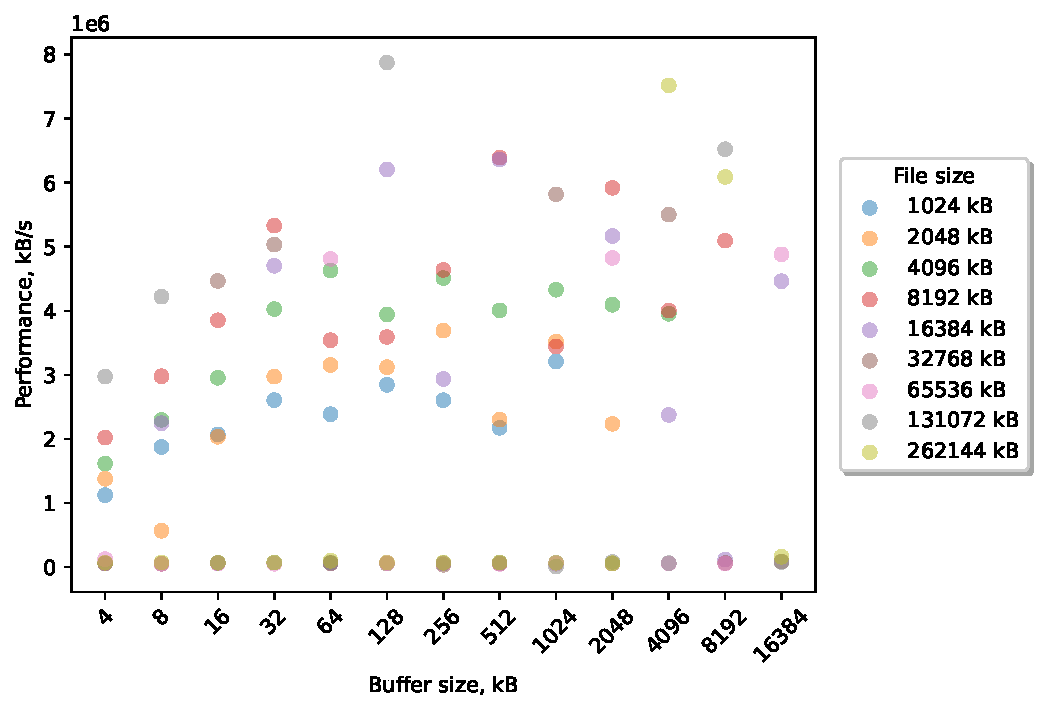
\includegraphics[width=1.0\textwidth]{figures.nosync/benchmarking/old/ffs/Read.pdf}
% 	\end{center}
% 	\caption{IOZone output for FFS Forward Read}
% \end{figure}

% \begin{figure}[!htb]
% 	\label{fig:app_bench_ffs_write}
% 	\begin{center}
% 		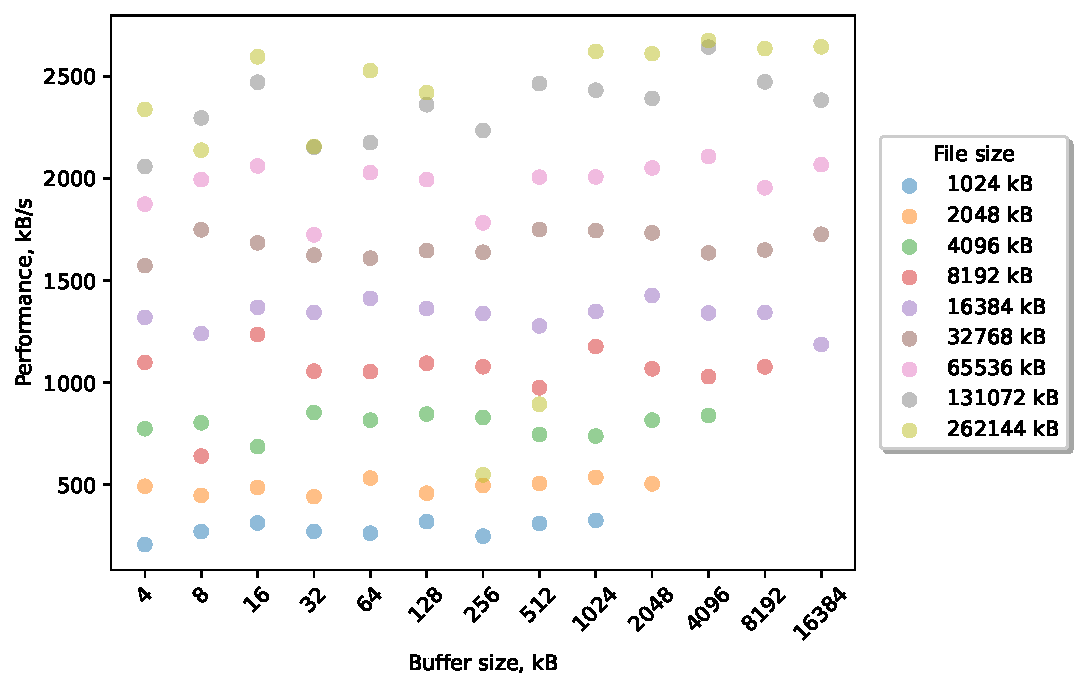
\includegraphics[width=1.0\textwidth]{figures.nosync/benchmarking/old/ffs/Write.pdf}
% 	\end{center}
% 	\caption{IOZone output for FFS Forward Write}
% \end{figure}

% \begin{figure}[!htb]
% 	\label{fig:app_bench_ffs_re_read}
% 	\begin{center}
% 		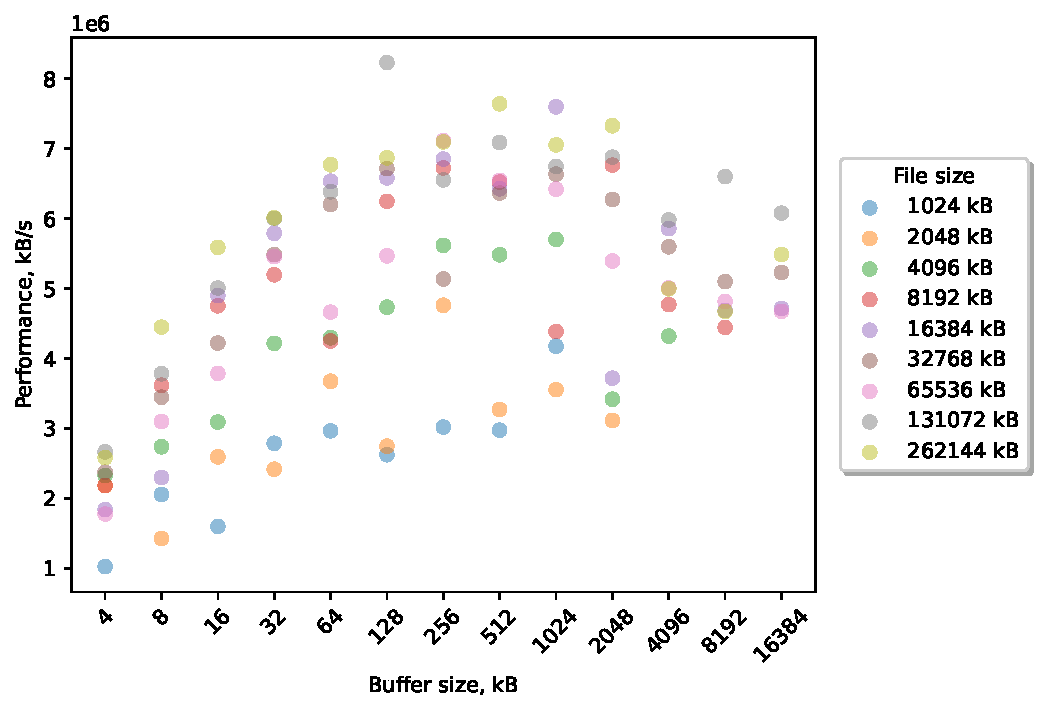
\includegraphics[width=1.0\textwidth]{figures.nosync/benchmarking/old/ffs/Re-Read.pdf}
% 	\end{center}
% 	\caption{IOZone output for FFS \mbox{Re-Read}}
% \end{figure}

% \begin{figure}[!htb]
% 	\label{fig:app_bench_ffs_re_write}
% 	\begin{center}
% 		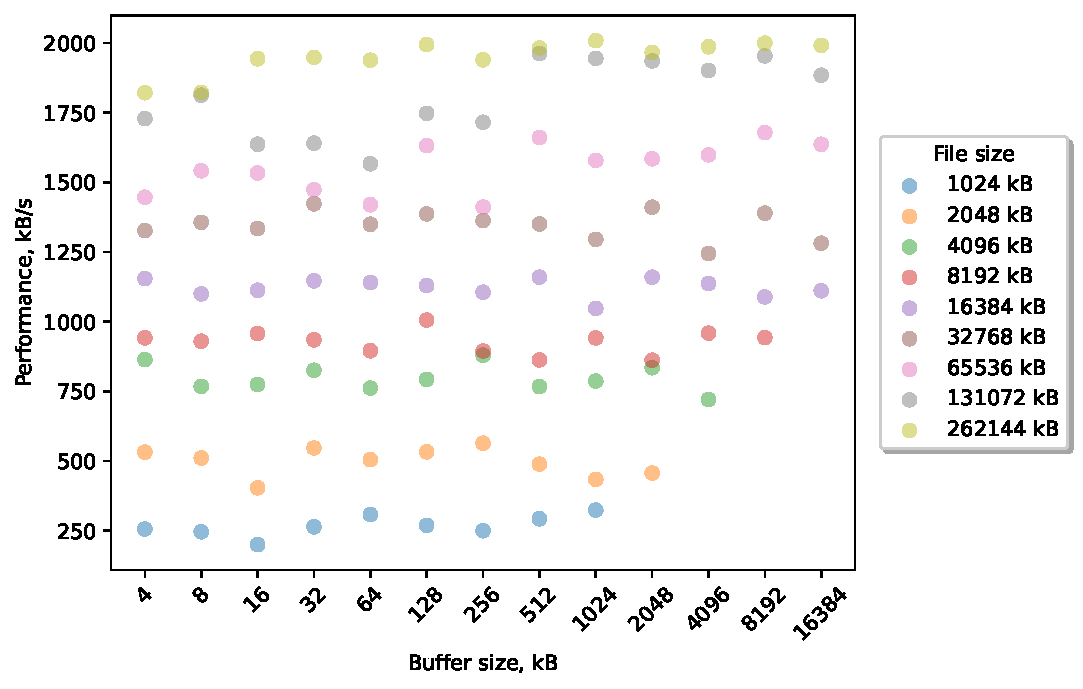
\includegraphics[width=1.0\textwidth]{figures.nosync/benchmarking/old/ffs/Re-Write.pdf}
% 	\end{center}
% 	\caption{IOZone output for FFS \mbox{Re-Write}}
% \end{figure}

% \begin{figure}[!htb]
% 	\label{fig:app_bench_ffs_rnd_read}
% 	\begin{center}
% 		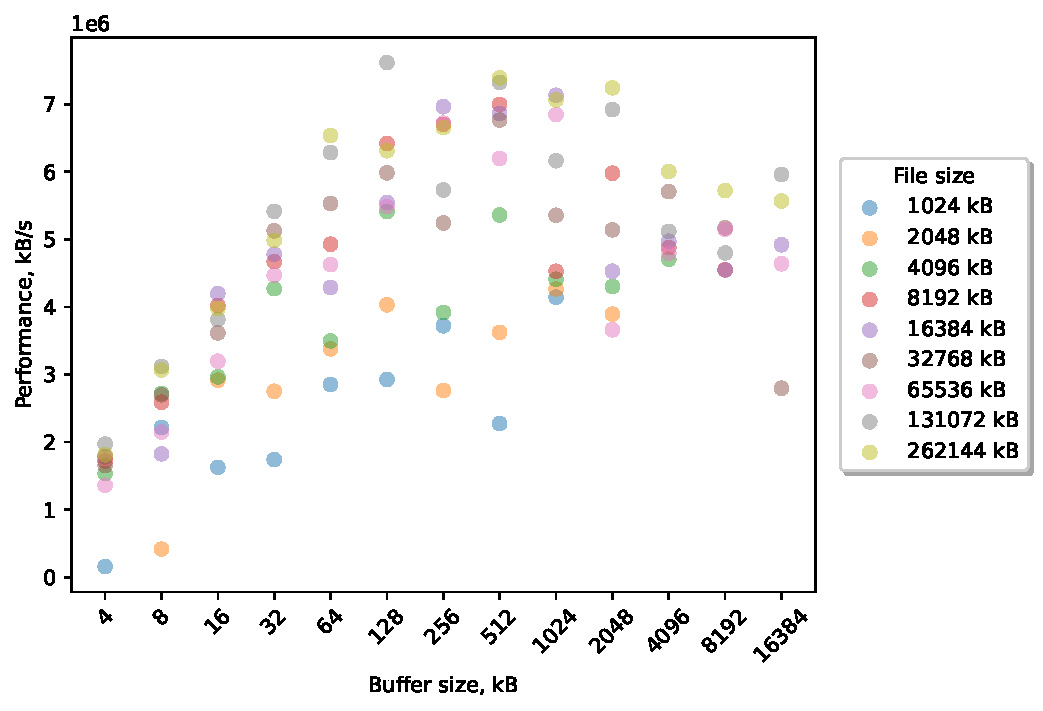
\includegraphics[width=1.0\textwidth]{figures.nosync/benchmarking/old/ffs/Random read.pdf}
% 	\end{center}
% 	\caption{IOZone output for FFS Random read}
% \end{figure}

% \begin{figure}[!htb]
% 	\label{fig:app_bench_ffs_rnd_write}
% 	\begin{center}
% 		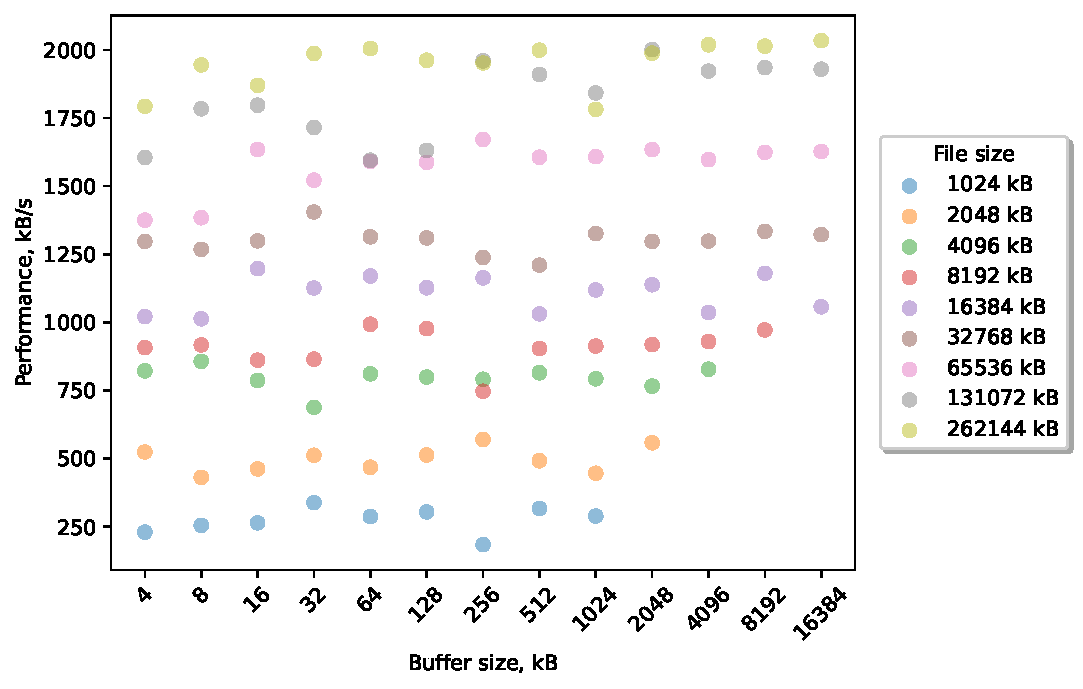
\includegraphics[width=1.0\textwidth]{figures.nosync/benchmarking/old/ffs/Random write.pdf}
% 	\end{center}
% 	\caption{IOZone output for FFS Random write}
% \end{figure}

\newpage

\section{GCSF}

\begin{table}[!ht]
	\begin{center}
		\caption{IOZone result for the Read test on GCSF in kilobytes per second}
		\resizebox{\textwidth}{!}{\begin{tabular}{| r | r | r | r | r | r | r | r | r | r | r | r | r | r | }
			
			\hline
			{} & \multicolumn{13}{c |}{Buffer size (kB)} \\
			\textbf{File size (kB)}   & \multicolumn{1}{c |}{4} & \multicolumn{1}{c |}{8} & \multicolumn{1}{c |}{16} & \multicolumn{1}{c |}{32} & \multicolumn{1}{c |}{64} & \multicolumn{1}{c |}{128} & \multicolumn{1}{c |}{256} & \multicolumn{1}{c |}{512} & \multicolumn{1}{c |}{1024} & \multicolumn{1}{c |}{2048} & \multicolumn{1}{c |}{4096} & \multicolumn{1}{c |}{8192} & \multicolumn{1}{c |}{16384}\\
			\hline
			\hline
			\textbf{1024}  & 1790460 & 2035716 & 2753527 & 3411938 & 3003881 & 3401130 & 3722435 & 4162573 & 4493556 & {} & {} & {} & {}\\
			\textbf{2048}  & 945007 & 2308622 & 3297725 & 4170264 & 3698085 & 2467800 & 3506373 & 4611288 & 5416763 & 4376355 & {} & {} & {}\\
			\textbf{4096}  & 1858527 & 2813233 & 1017897 & 4969868 & 4399673 & 4941279 & 4591331 & 5657217 & 5625724 & 5019235 & 3327622 & {} & {}\\
			\textbf{8192}  & 651866 & 480214 & 4126896 & 4664763 & 903994 & 5357988 & 3195123 & 5288712 & 6804170 & 1412655 & 4833405 & 5085204 & {}\\
			\textbf{16384}  & 409261 & 3463891 & 4768276 & 518677 & 5797739 & 6450228 & 6077171 & 6143453 & 6930296 & 6316241 & 5948808 & 837411 & 5326345\\
			\textbf{32768}  & 289995 & 2604351 & 514007 & 5222875 & 351689 & 380969 & 225834 & 428160 & 377558 & 3011251 & 422812 & 601160 & 710955\\
			\textbf{65536}  & 420968 & 390311 & 374191 & 590919 & 6243421 & 863782 & 388813 & 506734 & 463735 & 478777 & 456922 & 429282 & 624033\\
			\textbf{131072}  & 443068 & 462364 & 407350 & 496836 & 444001 & 471616 & 424145 & 518826 & 505112 & 559713 & 375452 & 526586 & 515828\\


			\hline

		\end{tabular}}
		\label{tbl:data_gcsf_read}
	\end{center}
\end{table}
	
\begin{table}[!ht]
	\begin{center}
		\caption{IOZone result for the Write test on GCSF in kilobytes per second}
		\resizebox{\textwidth}{!}{\begin{tabular}{| r | r | r | r | r | r | r | r | r | r | r | r | r | r | }
			
			\hline
			{} & \multicolumn{13}{c |}{Buffer size (kB)} \\
			\textbf{File size (kB)}   & \multicolumn{1}{c |}{4} & \multicolumn{1}{c |}{8} & \multicolumn{1}{c |}{16} & \multicolumn{1}{c |}{32} & \multicolumn{1}{c |}{64} & \multicolumn{1}{c |}{128} & \multicolumn{1}{c |}{256} & \multicolumn{1}{c |}{512} & \multicolumn{1}{c |}{1024} & \multicolumn{1}{c |}{2048} & \multicolumn{1}{c |}{4096} & \multicolumn{1}{c |}{8192} & \multicolumn{1}{c |}{16384}\\
			\hline
			\hline
			\textbf{1024}  & 489 & 517 & 445 & 461 & 399 & 496 & 509 & 448 & 529 & {} & {} & {} & {}\\
			\textbf{2048}  & 937 & 966 & 854 & 944 & 1072 & 966 & 944 & 954 & 868 & 969 & {} & {} & {}\\
			\textbf{4096}  & 1609 & 1614 & 1749 & 1607 & 1213 & 1787 & 1802 & 1519 & 1748 & 1551 & 1784 & {} & {}\\
			\textbf{8192}  & 3047 & 2233 & 2746 & 3115 & 2666 & 2636 & 3000 & 2974 & 3165 & 2716 & 3138 & 3122 & {}\\
			\textbf{16384}  & 4372 & 4180 & 4437 & 4690 & 4798 & 4642 & 4429 & 4781 & 4705 & 4670 & 4621 & 4875 & 4607\\
			\textbf{32768}  & 5377 & 6125 & 6471 & 6402 & 6343 & 6463 & 6435 & 6289 & 5865 & 6052 & 6317 & 6291 & 6018\\
			\textbf{65536}  & 6763 & 7448 & 7298 & 7825 & 6561 & 7061 & 7818 & 6959 & 7491 & 7706 & 5985 & 7343 & 6851\\
			\textbf{131072}  & 7276 & 7789 & 8553 & 8609 & 8243 & 8596 & 8168 & 8530 & 8596 & 8433 & 8029 & 8280 & 7959\\


			\hline

		\end{tabular}}
		\label{tbl:data_gcsf_write}
	\end{center}
\end{table}
	
\begin{table}[!ht]
	\begin{center}
		\caption{IOZone result for the Re-Read test on GCSF in kilobytes per second}
		\resizebox{\textwidth}{!}{\begin{tabular}{| r | r | r | r | r | r | r | r | r | r | r | r | r | r | }
			
			\hline
			{} & \multicolumn{13}{c |}{Buffer size (kB)} \\
			\textbf{File size (kB)}   & \multicolumn{1}{c |}{4} & \multicolumn{1}{c |}{8} & \multicolumn{1}{c |}{16} & \multicolumn{1}{c |}{32} & \multicolumn{1}{c |}{64} & \multicolumn{1}{c |}{128} & \multicolumn{1}{c |}{256} & \multicolumn{1}{c |}{512} & \multicolumn{1}{c |}{1024} & \multicolumn{1}{c |}{2048} & \multicolumn{1}{c |}{4096} & \multicolumn{1}{c |}{8192} & \multicolumn{1}{c |}{16384}\\
			\hline
			\hline
			\textbf{1024}  & 2632033 & 2187063 & 3200886 & 4304412 & 3348104 & 3778101 & 3281592 & 5048117 & 4083422 & {} & {} & {} & {}\\
			\textbf{2048}  & 2311728 & 3261415 & 4623699 & 4643695 & 4079167 & 4349761 & 6149699 & 6058611 & 7213548 & 5032754 & {} & {} & {}\\
			\textbf{4096}  & 2356697 & 2579635 & 4329816 & 5424983 & 5347310 & 6309619 & 4371684 & 6585338 & 6894546 & 6370451 & 5165626 & {} & {}\\
			\textbf{8192}  & 1891555 & 3974610 & 4017834 & 4884942 & 6112956 & 6262248 & 5158495 & 5116249 & 7087688 & 6720329 & 5270864 & 5038228 & {}\\
			\textbf{16384}  & 2228199 & 3960364 & 5075741 & 6187150 & 6473317 & 6838571 & 6919132 & 7139088 & 7211005 & 6614761 & 6187707 & 5016457 & 4594528\\
			\textbf{32768}  & 2503678 & 3836954 & 4593731 & 6020418 & 6336861 & 5357031 & 1864671 & 6139832 & 5652480 & 6276093 & 5945927 & 4010262 & 4741431\\
			\textbf{65536}  & 2639381 & 3531600 & 5031555 & 6133503 & 6445904 & 5921182 & 5961505 & 6217859 & 6461207 & 6398788 & 5278722 & 4674094 & 5364747\\
			\textbf{131072}  & 3039494 & 3904216 & 4889073 & 5950781 & 6275836 & 7495395 & 5875292 & 7344197 & 7196622 & 8031869 & 4689156 & 5687415 & 5207460\\


			\hline

		\end{tabular}}
		\label{tbl:data_gcsf_re-read}
	\end{center}
\end{table}
	
\begin{table}[!ht]
	\begin{center}
		\caption{IOZone result for the Re-Write test on GCSF in kilobytes per second}
		\resizebox{\textwidth}{!}{\begin{tabular}{| r | r | r | r | r | r | r | r | r | r | r | r | r | r | }
			
			\hline
			{} & \multicolumn{13}{c |}{Buffer size (kB)} \\
			\textbf{File size (kB)}   & \multicolumn{1}{c |}{4} & \multicolumn{1}{c |}{8} & \multicolumn{1}{c |}{16} & \multicolumn{1}{c |}{32} & \multicolumn{1}{c |}{64} & \multicolumn{1}{c |}{128} & \multicolumn{1}{c |}{256} & \multicolumn{1}{c |}{512} & \multicolumn{1}{c |}{1024} & \multicolumn{1}{c |}{2048} & \multicolumn{1}{c |}{4096} & \multicolumn{1}{c |}{8192} & \multicolumn{1}{c |}{16384}\\
			\hline
			\hline
			\textbf{1024}  & 371 & 330 & 295 & 433 & 400 & 329 & 259 & 335 & 409 & {} & {} & {} & {}\\
			\textbf{2048}  & 550 & 612 & 738 & 736 & 814 & 775 & 600 & 592 & 799 & 787 & {} & {} & {}\\
			\textbf{4096}  & 873 & 1354 & 1503 & 1239 & 927 & 1317 & 1368 & 1342 & 1424 & 1277 & 1325 & {} & {}\\
			\textbf{8192}  & 1118 & 2201 & 1192 & 2117 & 1883 & 2093 & 2004 & 2126 & 1877 & 2192 & 2014 & 2165 & {}\\
			\textbf{16384}  & 1370 & 2949 & 2955 & 2963 & 2678 & 2950 & 2974 & 3018 & 3134 & 2989 & 2827 & 3067 & 1401\\
			\textbf{32768}  & 3354 & 3448 & 3200 & 3592 & 3656 & 3815 & 3532 & 3702 & 3629 & 3675 & 3508 & 3708 & 3621\\
			\textbf{65536}  & 3815 & 3962 & 3849 & 2319 & 3794 & 4085 & 3970 & 4080 & 3929 & 4033 & 3787 & 2972 & 4044\\
			\textbf{131072}  & 4443 & 4682 & 4721 & 4807 & 4749 & 4866 & 4774 & 4766 & 4683 & 4760 & 4623 & 4657 & 4804\\


			\hline

		\end{tabular}}
		\label{tbl:data_gcsf_re-write}
	\end{center}
\end{table}
	
\begin{table}[!ht]
	\begin{center}
		\caption{IOZone result for the Random read test on GCSF in kilobytes per second}
		\resizebox{\textwidth}{!}{\begin{tabular}{| r | r | r | r | r | r | r | r | r | r | r | r | r | r | }
			
			\hline
			{} & \multicolumn{13}{c |}{Buffer size (kB)} \\
			\textbf{File size (kB)}   & \multicolumn{1}{c |}{4} & \multicolumn{1}{c |}{8} & \multicolumn{1}{c |}{16} & \multicolumn{1}{c |}{32} & \multicolumn{1}{c |}{64} & \multicolumn{1}{c |}{128} & \multicolumn{1}{c |}{256} & \multicolumn{1}{c |}{512} & \multicolumn{1}{c |}{1024} & \multicolumn{1}{c |}{2048} & \multicolumn{1}{c |}{4096} & \multicolumn{1}{c |}{8192} & \multicolumn{1}{c |}{16384}\\
			\hline
			\hline
			\textbf{1024}  & 1992279 & 1741104 & 3923040 & 2892612 & 3284101 & 2875184 & 4282950 & 3684119 & 3179559 & {} & {} & {} & {}\\
			\textbf{2048}  & 2122645 & 2592166 & 2843590 & 5006356 & 4221501 & 4481379 & 6583305 & 5200329 & 7343043 & 4934459 & {} & {} & {}\\
			\textbf{4096}  & 1723189 & 2471992 & 4007615 & 4899008 & 5625724 & 5713661 & 6503078 & 6897314 & 4958393 & 5270212 & 5063617 & {} & {}\\
			\textbf{8192}  & 1438199 & 3111222 & 4149824 & 5095007 & 5821902 & 5885728 & 4543853 & 6350207 & 7173514 & 6501608 & 5372229 & 4654652 & {}\\
			\textbf{16384}  & 1859705 & 2912112 & 4175240 & 5158807 & 6039252 & 6725463 & 6203907 & 6921919 & 6820923 & 6546080 & 5667676 & 5441055 & 5336686\\
			\textbf{32768}  & 1705159 & 2794224 & 4285618 & 5467855 & 5548200 & 6087347 & 6091664 & 5991547 & 5893405 & 6215636 & 6222672 & 3776853 & 5156254\\
			\textbf{65536}  & 1843064 & 2695626 & 4393982 & 4975003 & 6203125 & 5990477 & 4676082 & 7062855 & 6735419 & 6700285 & 4143421 & 4907587 & 5587993\\
			\textbf{131072}  & 2100647 & 2842719 & 3678063 & 5056629 & 5706720 & 6765741 & 5708261 & 7233171 & 7090347 & 7451506 & 4198987 & 5471360 & 5404768\\


			\hline

		\end{tabular}}
		\label{tbl:data_gcsf_random_read}
	\end{center}
\end{table}
	
\begin{table}[!ht]
	\begin{center}
		\caption{IOZone result for the Random write test on GCSF in kilobytes per second}
		\resizebox{\textwidth}{!}{\begin{tabular}{| r | r | r | r | r | r | r | r | r | r | r | r | r | r | }
			
			\hline
			{} & \multicolumn{13}{c |}{Buffer size (kB)} \\
			\textbf{File size (kB)}   & \multicolumn{1}{c |}{4} & \multicolumn{1}{c |}{8} & \multicolumn{1}{c |}{16} & \multicolumn{1}{c |}{32} & \multicolumn{1}{c |}{64} & \multicolumn{1}{c |}{128} & \multicolumn{1}{c |}{256} & \multicolumn{1}{c |}{512} & \multicolumn{1}{c |}{1024} & \multicolumn{1}{c |}{2048} & \multicolumn{1}{c |}{4096} & \multicolumn{1}{c |}{8192} & \multicolumn{1}{c |}{16384}\\
			\hline
			\hline
			\textbf{1024}  & 373 & 338 & 295 & 364 & 355 & 222 & 368 & 404 & 410 & {} & {} & {} & {}\\
			\textbf{2048}  & 739 & 784 & 753 & 789 & 852 & 823 & 688 & 741 & 639 & 657 & {} & {} & {}\\
			\textbf{4096}  & 958 & 1418 & 1299 & 1372 & 812 & 884 & 1369 & 1330 & 1416 & 1194 & 1335 & {} & {}\\
			\textbf{8192}  & 2200 & 2310 & 2289 & 2445 & 2174 & 2195 & 2106 & 2043 & 2063 & 1962 & 2111 & 2195 & {}\\
			\textbf{16384}  & 2739 & 2747 & 3476 & 3141 & 3478 & 2894 & 3123 & 2949 & 3054 & 2925 & 2941 & 2911 & 1223\\
			\textbf{32768}  & 2567 & 3154 & 3766 & 4474 & 3738 & 4330 & 3664 & 3798 & 3534 & 3745 & 3675 & 3732 & 3613\\
			\textbf{65536}  & 2646 & 2769 & 3422 & 4011 & 4985 & 4159 & 5019 & 3739 & 4051 & 3962 & 3899 & 4087 & 4193\\
			\textbf{131072}  & 2124 & 3073 & 3481 & 4239 & 5025 & 6502 & 5285 & 6129 & 4806 & 4689 & 4747 & 4834 & 4832\\


			\hline

		\end{tabular}}
		\label{tbl:data_gcsf_random_write}
	\end{center}
\end{table}
	

\FloatBarrier
% \begin{figure}[!htb]
% 	\label{fig:app_bgcsfh_ffs_read}
% 	\begin{center}
% 		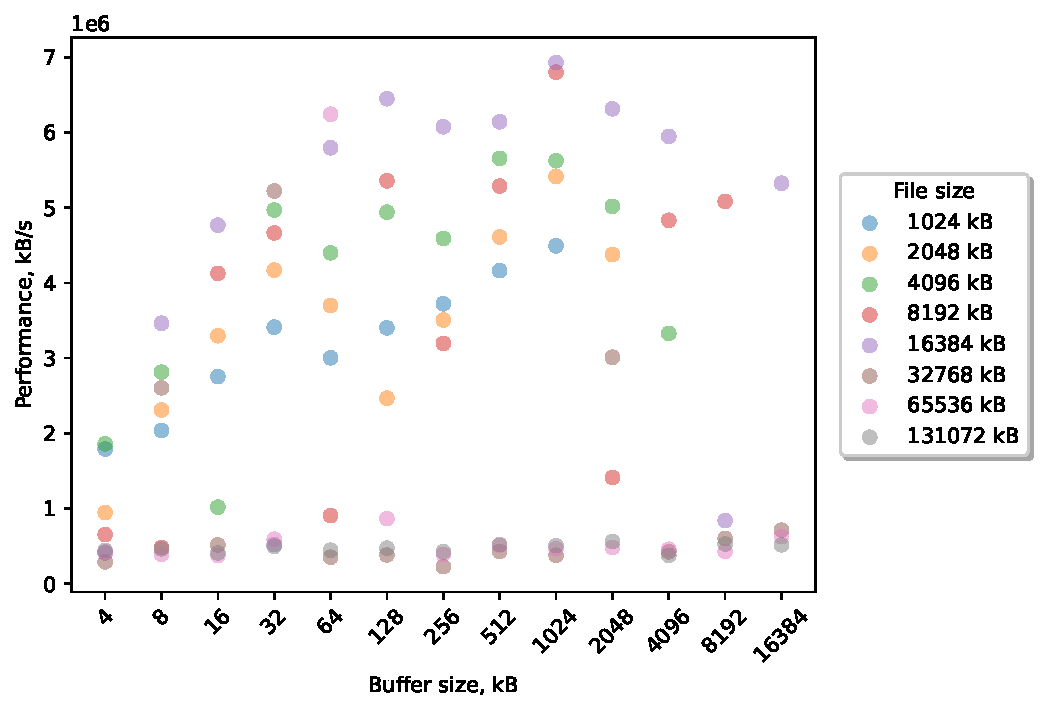
\includegraphics[width=1.0\textwidth]{figures.nosync/benchmarking/old/gcsf/Read.pdf}
% 	\end{center}
% 	\caption{IOZone output for GCSF Forward Read}
% \end{figure}

% \begin{figure}[!htb]
% 	\label{fig:app_begcsf_ffs_write}
% 	\begin{center}
% 		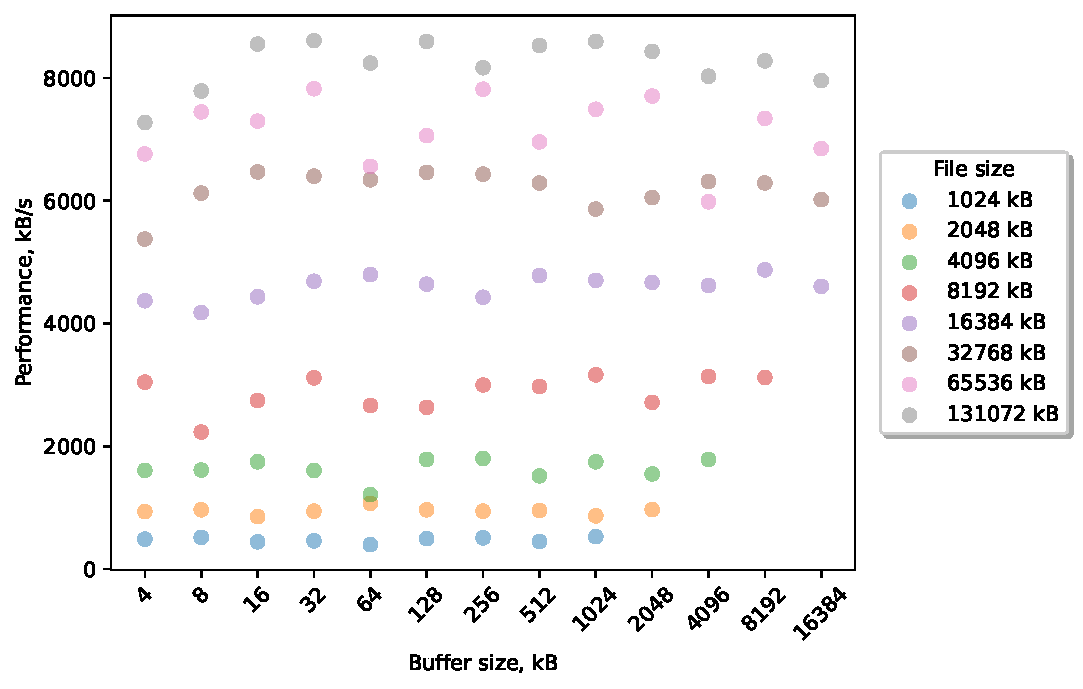
\includegraphics[width=1.0\textwidth]{figures.nosync/benchmarking/old/gcsf/Write.pdf}
% 	\end{center}
% 	\caption{IOZone output for GCSF Forward Write}
% \end{figure}

% \begin{figure}[!htb]
% 	\label{fig:app_bencgcsffs_re_read}
% 	\begin{center}
% 		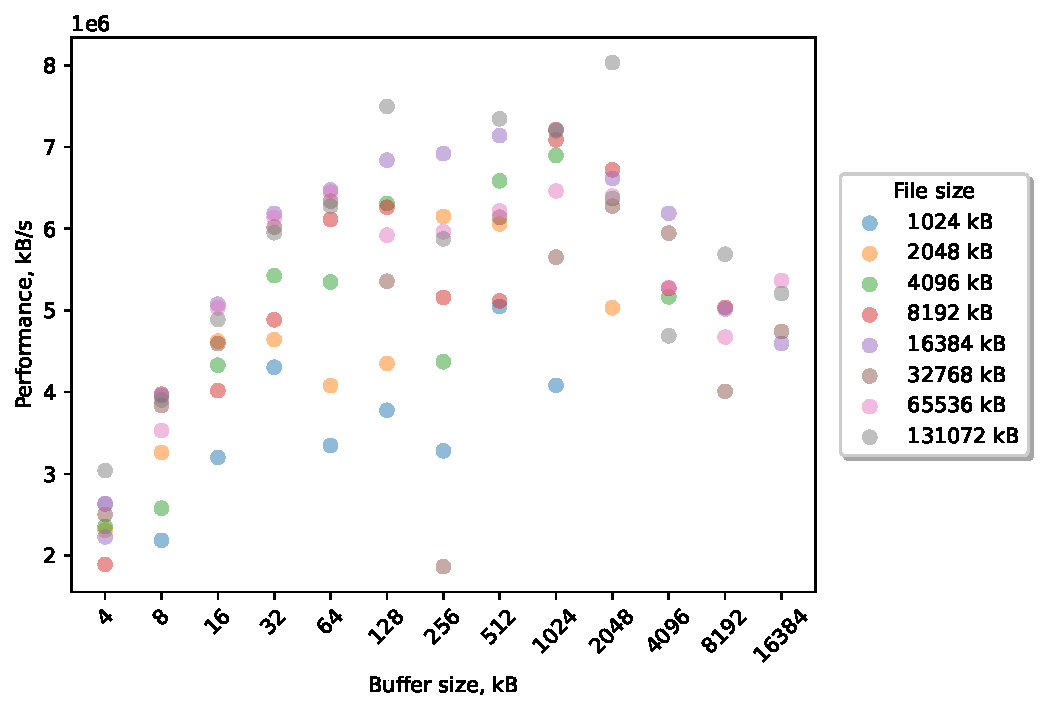
\includegraphics[width=1.0\textwidth]{figures.nosync/benchmarking/old/gcsf/Re-Read.pdf}
% 	\end{center}
% 	\caption{IOZone output for GCSF \mbox{Re-Read}}
% \end{figure}

% \begin{figure}[!htb]
% 	\label{fig:app_benchgcsfs_re_write}
% 	\begin{center}
% 		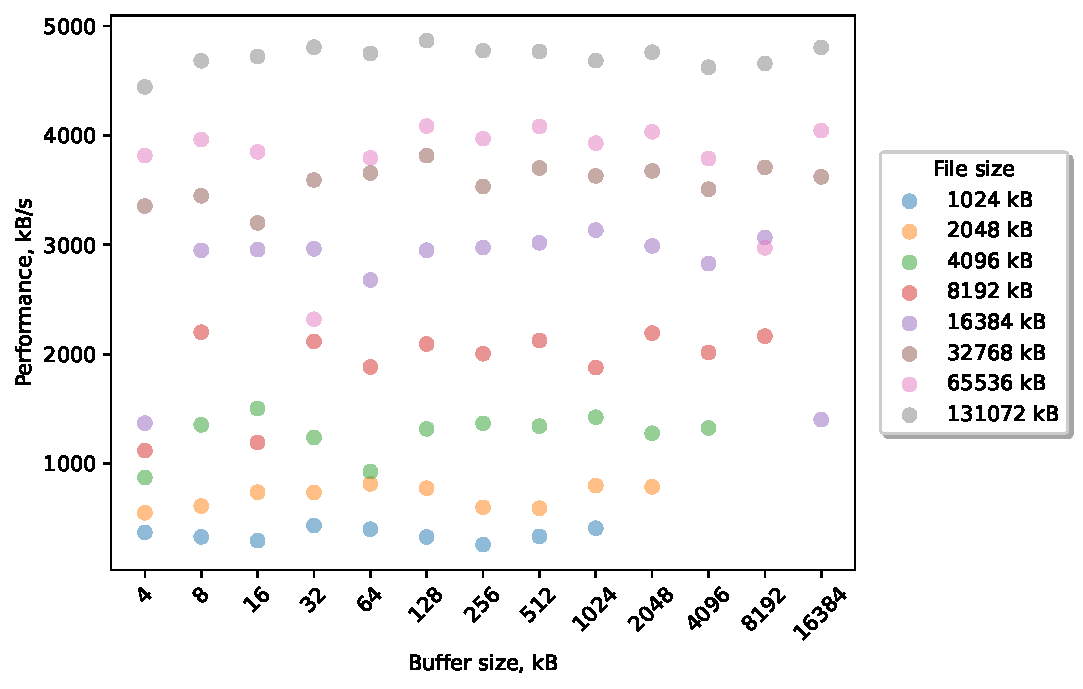
\includegraphics[width=1.0\textwidth]{figures.nosync/benchmarking/old/gcsf/Re-Write.pdf}
% 	\end{center}
% 	\caption{IOZone output for GCSF \mbox{Re-Write}}
% \end{figure}

% \begin{figure}[!htb]
% 	\label{fig:app_benchgcsfs_rnd_read}
% 	\begin{center}
% 		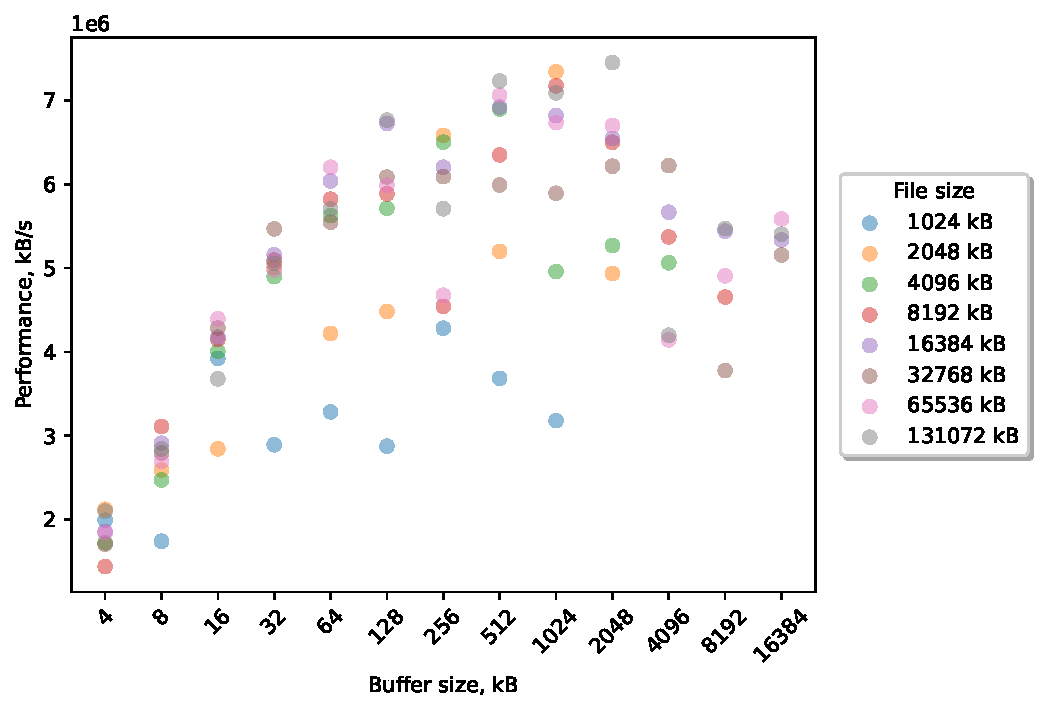
\includegraphics[width=1.0\textwidth]{figures.nosync/benchmarking/old/gcsf/Random read.pdf}
% 	\end{center}
% 	\caption{IOZone output for GCSF Random read}
% \end{figure}

% \begin{figure}[!htb]
% 	\label{fig:app_bench_gcsf_rnd_write}
% 	\begin{center}
% 		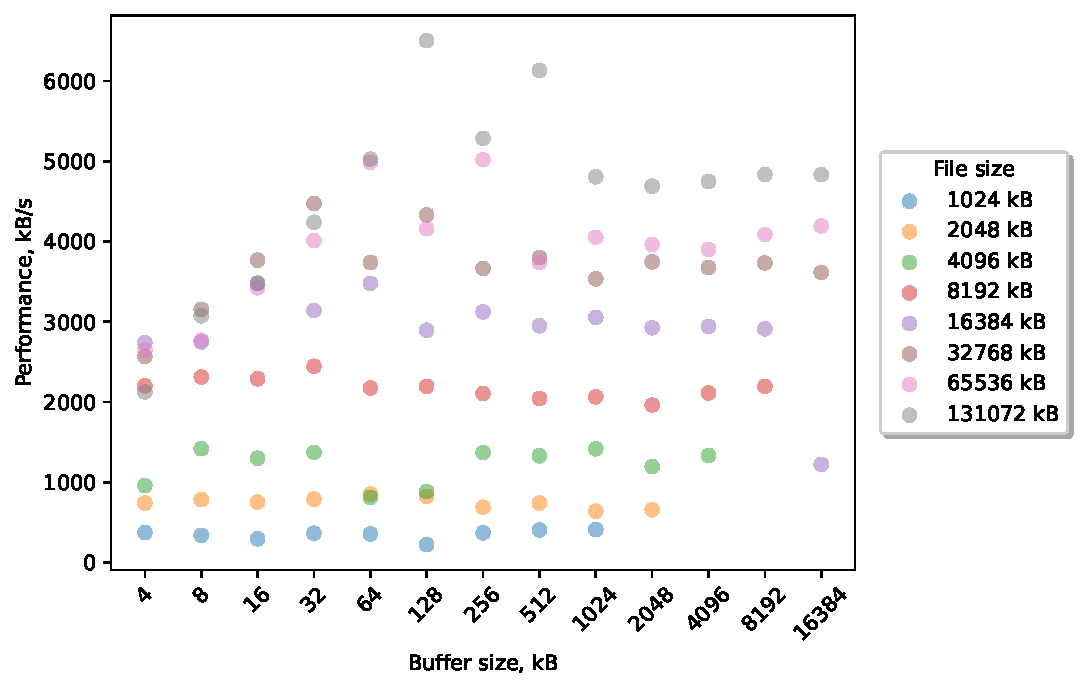
\includegraphics[width=1.0\textwidth]{figures.nosync/benchmarking/old/gcsf/Random write.pdf}
% 	\end{center}
% 	\caption{IOZone output for GCSF Random write}
% \end{figure}

\newpage

\section{Fejk FFS}

\begin{table}[!ht]
	\begin{center}
		\caption{IOZone result for the Read test on FFFS in kilobytes per second}
		\resizebox{\textwidth}{!}{\begin{tabular}{| r | r | r | r | r | r | r | r | r | r | r | r | r | r | }
			
			\hline
			{} & \multicolumn{13}{c |}{Buffer size (kB)} \\
			\textbf{File size (kB)}   & \multicolumn{1}{c |}{4} & \multicolumn{1}{c |}{8} & \multicolumn{1}{c |}{16} & \multicolumn{1}{c |}{32} & \multicolumn{1}{c |}{64} & \multicolumn{1}{c |}{128} & \multicolumn{1}{c |}{256} & \multicolumn{1}{c |}{512} & \multicolumn{1}{c |}{1024} & \multicolumn{1}{c |}{2048} & \multicolumn{1}{c |}{4096} & \multicolumn{1}{c |}{8192} & \multicolumn{1}{c |}{16384}\\
			\hline
			\hline
			\textbf{1024}  & 1605111 & 2472911 & 889631 & 2715230 & 3618930 & 3001782 & 1032244 & 2578312 & 2467229 & {} & {} & {} & {}\\
			\textbf{2048}  & 1921339 & 1930406 & 2194777 & 2821176 & 3200654 & 4130162 & 4154130 & 2649737 & 5032754 & 3286370 & {} & {} & {}\\
			\textbf{4096}  & 2426601 & 2784507 & 3271230 & 3574071 & 3670280 & 5542240 & 4386193 & 3771811 & 3995498 & 4763181 & 4000150 & {} & {}\\
			\textbf{8192}  & 2895693 & 3535750 & 4173008 & 5378957 & 4899570 & 4548665 & 5914094 & 6558696 & 4271046 & 4104220 & 5475825 & 5888754 & {}\\
			\textbf{16384}  & 3094244 & 4152032 & 4908602 & 3512941 & 6234299 & 5855539 & 6313919 & 7272051 & 6212881 & 7111751 & 5507336 & 5387732 & 5486670\\
			\textbf{32768}  & 2848900 & 3537882 & 4681672 & 6104381 & 6554760 & 5933093 & 6802626 & 6375072 & 6339199 & 6146697 & 6030191 & 5591994 & 5440583\\
			\textbf{65536}  & 70116 & 3562495 & 5159913 & 5999237 & 7335592 & 7026566 & 7648924 & 6445904 & 77043 & 129764 & 5783761 & 5526649 & 4978066\\
			\textbf{131072}  & 394463 & 2034461 & 454646 & 6311863 & 3782086 & 280028 & 7525973 & 6890568 & 75477 & 59220 & 2674224 & 238745 & 657556\\
			\textbf{262144}  & 65486 & 75529 & 77854 & 97658 & 79916 & 72736 & 76276 & 71780 & 106689 & 72269 & 72176 & 79924 & 126614\\


			\hline

		\end{tabular}}
		\label{tbl:data_fejk-ffs_read}
	\end{center}
\end{table}
	
\begin{table}[!ht]
	\begin{center}
		\caption{IOZone result for the Write test on FFFS in kilobytes per second}
		\resizebox{\textwidth}{!}{\begin{tabular}{| r | r | r | r | r | r | r | r | r | r | r | r | r | r | }
			
			\hline
			{} & \multicolumn{13}{c |}{Buffer size (kB)} \\
			\textbf{File size (kB)}   & \multicolumn{1}{c |}{4} & \multicolumn{1}{c |}{8} & \multicolumn{1}{c |}{16} & \multicolumn{1}{c |}{32} & \multicolumn{1}{c |}{64} & \multicolumn{1}{c |}{128} & \multicolumn{1}{c |}{256} & \multicolumn{1}{c |}{512} & \multicolumn{1}{c |}{1024} & \multicolumn{1}{c |}{2048} & \multicolumn{1}{c |}{4096} & \multicolumn{1}{c |}{8192} & \multicolumn{1}{c |}{16384}\\
			\hline
			\hline
			\textbf{1024}  & 5193 & 5287 & 4303 & 5160 & 5076 & 5282 & 27847 & 5736 & 5086 & {} & {} & {} & {}\\
			\textbf{2048}  & 4807 & 5335 & 4665 & 6305 & 6258 & 5920 & 6228 & 6453 & 5811 & 6301 & {} & {} & {}\\
			\textbf{4096}  & 5767 & 5943 & 5979 & 5807 & 6265 & 6320 & 3784 & 6770 & 5759 & 6188 & 6844 & {} & {}\\
			\textbf{8192}  & 5504 & 6464 & 6702 & 6783 & 6175 & 6015 & 5288 & 6874 & 98659 & 101980 & 7043 & 6738 & {}\\
			\textbf{16384}  & 6430 & 6955 & 7463 & 7442 & 6794 & 7637 & 7667 & 7628 & 7337 & 101677 & 7553 & 7824 & 7735\\
			\textbf{32768}  & 7232 & 7656 & 7808 & 7859 & 8075 & 8142 & 8075 & 8062 & 8161 & 7896 & 8229 & 117474 & 8377\\
			\textbf{65536}  & 7370 & 7246 & 7273 & 7350 & 7530 & 7664 & 7658 & 8170 & 6959 & 7196 & 7192 & 7019 & 6735\\
			\textbf{131072}  & 7160 & 6974 & 6961 & 7229 & 7593 & 7217 & 7901 & 8196 & 8116 & 5763 & 7398 & 5990 & 8025\\
			\textbf{262144}  & 7167 & 7419 & 7937 & 7545 & 8435 & 8520 & 8030 & 7742 & 3996 & 7468 & 7601 & 8066 & 7891\\
			\textbf{524288}  & 7578 & 7967 & 8161 & 82 & 8189 & 8494 & 8454 & 8327 & 8466 & 8501 & 8370 & 8308 & 5935\\


			\hline

		\end{tabular}}
		\label{tbl:data_fejk-ffs_write}
	\end{center}
\end{table}
	
\begin{table}[!ht]
	\begin{center}
		\caption{IOZone result for the Re-Read test on FFFS in kilobytes per second}
		\resizebox{\textwidth}{!}{\begin{tabular}{| r | r | r | r | r | r | r | r | r | r | r | r | r | r | }
			
			\hline
			{} & \multicolumn{13}{c |}{Buffer size (kB)} \\
			\textbf{File size (kB)}   & \multicolumn{1}{c |}{4} & \multicolumn{1}{c |}{8} & \multicolumn{1}{c |}{16} & \multicolumn{1}{c |}{32} & \multicolumn{1}{c |}{64} & \multicolumn{1}{c |}{128} & \multicolumn{1}{c |}{256} & \multicolumn{1}{c |}{512} & \multicolumn{1}{c |}{1024} & \multicolumn{1}{c |}{2048} & \multicolumn{1}{c |}{4096} & \multicolumn{1}{c |}{8192} & \multicolumn{1}{c |}{16384}\\
			\hline
			\hline
			\textbf{1024}  & 1984913 & 2820430 & 2353657 & 4674510 & 4232305 & 3198502 & 1920993 & 4943530 & 3142339 & {} & {} & {} & {}\\
			\textbf{2048}  & 2107025 & 3011047 & 2367151 & 3915540 & 4633675 & 5209791 & 5119743 & 4663865 & 4829046 & 3736694 & {} & {} & {}\\
			\textbf{4096}  & 3075079 & 3614679 & 4462528 & 4302706 & 5971855 & 6503078 & 4906002 & 6471234 & 4132949 & 5184332 & 3442303 & {} & {}\\
			\textbf{8192}  & 2826843 & 4114541 & 4678737 & 5261179 & 4158362 & 6182248 & 5094251 & 5357152 & 6537482 & 5382328 & 5756551 & 5915112 & {}\\
			\textbf{16384}  & 3115426 & 4517212 & 5147601 & 6343059 & 6609036 & 6262707 & 6753222 & 7984318 & 6787239 & 7246745 & 5728625 & 5310703 & 5452279\\
			\textbf{32768}  & 2786858 & 3742299 & 5009656 & 7004755 & 7299786 & 7123475 & 7777741 & 6994062 & 6752162 & 7039557 & 6382473 & 5967613 & 5664360\\
			\textbf{65536}  & 2205856 & 4396090 & 5428742 & 6393876 & 6889031 & 6089074 & 7811071 & 6860318 & 7461842 & 6801920 & 6440769 & 5750246 & 4823451\\
			\textbf{131072}  & 3287977 & 3847707 & 5198793 & 6348527 & 6951999 & 8443258 & 7909267 & 7114111 & 7388515 & 5298401 & 3139222 & 5802490 & 6479087\\
			\textbf{262144}  & 2974653 & 4452026 & 5376537 & 6145825 & 7115944 & 7217446 & 7116911 & 6533364 & 6027138 & 6506108 & 5360469 & 5598732 & 5819467\\


			\hline

		\end{tabular}}
		\label{tbl:data_fejk-ffs_re-read}
	\end{center}
\end{table}
	
\begin{table}[!ht]
	\begin{center}
		\caption{IOZone result for the Re-Write test on FFFS in kilobytes per second}
		\resizebox{\textwidth}{!}{\begin{tabular}{| r | r | r | r | r | r | r | r | r | r | r | r | r | r | }
			
			\hline
			{} & \multicolumn{13}{c |}{Buffer size (kB)} \\
			\textbf{File size (kB)}   & \multicolumn{1}{c |}{4} & \multicolumn{1}{c |}{8} & \multicolumn{1}{c |}{16} & \multicolumn{1}{c |}{32} & \multicolumn{1}{c |}{64} & \multicolumn{1}{c |}{128} & \multicolumn{1}{c |}{256} & \multicolumn{1}{c |}{512} & \multicolumn{1}{c |}{1024} & \multicolumn{1}{c |}{2048} & \multicolumn{1}{c |}{4096} & \multicolumn{1}{c |}{8192} & \multicolumn{1}{c |}{16384}\\
			\hline
			\hline
			\textbf{1024}  & 4574 & 4975 & 1566 & 5157 & 4391 & 4913 & 3380 & 27982 & 5001 & {} & {} & {} & {}\\
			\textbf{2048}  & 3371 & 4654 & 5206 & 4614 & 5631 & 5635 & 5680 & 31266 & 5577 & 5685 & {} & {} & {}\\
			\textbf{4096}  & 5548 & 5728 & 5588 & 5188 & 5330 & 5148 & 5077 & 5928 & 5449 & 4753 & 5515 & {} & {}\\
			\textbf{8192}  & 5296 & 5167 & 5574 & 5177 & 5002 & 5540 & 5362 & 5527 & 5913 & 5893 & 5485 & 4895 & {}\\
			\textbf{16384}  & 5933 & 5866 & 6309 & 6263 & 5714 & 6230 & 6215 & 6563 & 6454 & 6412 & 5640 & 25482 & 6565\\
			\textbf{32768}  & 6314 & 6369 & 6575 & 6687 & 6841 & 6852 & 6824 & 6819 & 6889 & 6768 & 6782 & 6699 & 6885\\
			\textbf{65536}  & 5933 & 6327 & 5753 & 6290 & 6514 & 5615 & 6329 & 6632 & 5962 & 5815 & 5749 & 5935 & 25761\\
			\textbf{131072}  & 5885 & 5619 & 6099 & 6598 & 6601 & 5990 & 6717 & 6763 & 5816 & 4048 & 6124 & 4737 & 6436\\
			\textbf{262144}  & 5769 & 6203 & 6474 & 6722 & 6879 & 6865 & 6565 & 6140 & 6177 & 6033 & 6164 & 6586 & 6653\\


			\hline

		\end{tabular}}
		\label{tbl:data_fejk-ffs_re-write}
	\end{center}
\end{table}
	
\begin{table}[!ht]
	\begin{center}
		\caption{IOZone result for the Random read test on FFFS in kilobytes per second}
		\resizebox{\textwidth}{!}{\begin{tabular}{| r | r | r | r | r | r | r | r | r | r | r | r | r | r | }
			
			\hline
			{} & \multicolumn{13}{c |}{Buffer size (kB)} \\
			\textbf{File size (kB)}   & \multicolumn{1}{c |}{4} & \multicolumn{1}{c |}{8} & \multicolumn{1}{c |}{16} & \multicolumn{1}{c |}{32} & \multicolumn{1}{c |}{64} & \multicolumn{1}{c |}{128} & \multicolumn{1}{c |}{256} & \multicolumn{1}{c |}{512} & \multicolumn{1}{c |}{1024} & \multicolumn{1}{c |}{2048} & \multicolumn{1}{c |}{4096} & \multicolumn{1}{c |}{8192} & \multicolumn{1}{c |}{16384}\\
			\hline
			\hline
			\textbf{1024}  & 1438461 & 2474336 & 3335105 & 4339202 & 4574926 & 3594699 & 1662264 & 4415030 & 3390391 & {} & {} & {} & {}\\
			\textbf{2048}  & 1639674 & 2531808 & 2980747 & 3071337 & 4971585 & 5626082 & 5235193 & 4240255 & 3864455 & 4591569 & {} & {} & {}\\
			\textbf{4096}  & 2333965 & 2898672 & 4076076 & 4214051 & 3641495 & 6716643 & 3128843 & 6022095 & 4428023 & 4935601 & 5551194 & {} & {}\\
			\textbf{8192}  & 2217071 & 1882745 & 4242044 & 6006101 & 3655755 & 6054786 & 6947247 & 6912307 & 6339662 & 5785631 & 5789530 & 5583494 & {}\\
			\textbf{16384}  & 2235520 & 2613523 & 4010753 & 5637917 & 5897753 & 5362924 & 6542963 & 7922644 & 6671272 & 7117644 & 4702688 & 5233056 & 5189585\\
			\textbf{32768}  & 1953956 & 2985674 & 4118168 & 6358850 & 7157605 & 6732647 & 7552086 & 7015482 & 6541968 & 7126430 & 6545707 & 5985025 & 5650853\\
			\textbf{65536}  & 1320279 & 3522910 & 4420978 & 5494832 & 6317898 & 6091233 & 7578280 & 6635907 & 7317626 & 6684480 & 6613236 & 5663404 & 4218907\\
			\textbf{131072}  & 2179297 & 3011967 & 4211016 & 5669935 & 6324062 & 7899720 & 7685258 & 6951208 & 7292757 & 5564284 & 2867974 & 5863448 & 6536945\\
			\textbf{262144}  & 2105727 & 3331986 & 4265958 & 5398262 & 6599796 & 7121152 & 6889437 & 6293359 & 6270783 & 5819868 & 5256751 & 5823875 & 5831010\\


			\hline

		\end{tabular}}
		\label{tbl:data_fejk-ffs_random_read}
	\end{center}
\end{table}
	
\begin{table}[!ht]
	\begin{center}
		\caption{IOZone result for the Random write test on FFFS in kilobytes per second}
		\resizebox{\textwidth}{!}{\begin{tabular}{| r | r | r | r | r | r | r | r | r | r | r | r | r | r | }
			
			\hline
			{} & \multicolumn{13}{c |}{Buffer size (kB)} \\
			\textbf{File size (kB)}   & \multicolumn{1}{c |}{4} & \multicolumn{1}{c |}{8} & \multicolumn{1}{c |}{16} & \multicolumn{1}{c |}{32} & \multicolumn{1}{c |}{64} & \multicolumn{1}{c |}{128} & \multicolumn{1}{c |}{256} & \multicolumn{1}{c |}{512} & \multicolumn{1}{c |}{1024} & \multicolumn{1}{c |}{2048} & \multicolumn{1}{c |}{4096} & \multicolumn{1}{c |}{8192} & \multicolumn{1}{c |}{16384}\\
			\hline
			\hline
			\textbf{1024}  & 4619 & 4008 & 2880 & 4530 & 4425 & 4764 & 3097 & 5879 & 4465 & {} & {} & {} & {}\\
			\textbf{2048}  & 4620 & 4691 & 5179 & 5665 & 5728 & 5660 & 4573 & 5554 & 5775 & 5519 & {} & {} & {}\\
			\textbf{4096}  & 5284 & 5681 & 5333 & 5194 & 5488 & 5822 & 5854 & 6127 & 37216 & 5145 & 5738 & {} & {}\\
			\textbf{8192}  & 5442 & 4747 & 5737 & 5386 & 5800 & 5088 & 5881 & 5811 & 5414 & 5708 & 4852 & 5635 & {}\\
			\textbf{16384}  & 5553 & 6011 & 6191 & 6267 & 6188 & 5654 & 6348 & 6585 & 6428 & 6509 & 5831 & 6558 & 6496\\
			\textbf{32768}  & 6253 & 6238 & 6434 & 6511 & 6810 & 6829 & 6984 & 6800 & 6877 & 6801 & 6853 & 6875 & 6857\\
			\textbf{65536}  & 4967 & 6318 & 5379 & 5753 & 6616 & 6361 & 6528 & 6611 & 5854 & 5900 & 5980 & 6472 & 5881\\
			\textbf{131072}  & 5754 & 5611 & 6114 & 6317 & 6102 & 6407 & 6469 & 6662 & 4629 & 4861 & 5661 & 5536 & 6443\\
			\textbf{262144}  & 5741 & 6259 & 6439 & 6689 & 6907 & 6427 & 6463 & 6100 & 6309 & 5998 & 6035 & 6849 & 6857\\


			\hline

		\end{tabular}}
		\label{tbl:data_fejk-ffs_random_write}
	\end{center}
\end{table}
	

\FloatBarrier
% \begin{figure}[!htb]
% 	\label{fig:app_bencfh_ffs_read}
% 	\begin{center}
% 		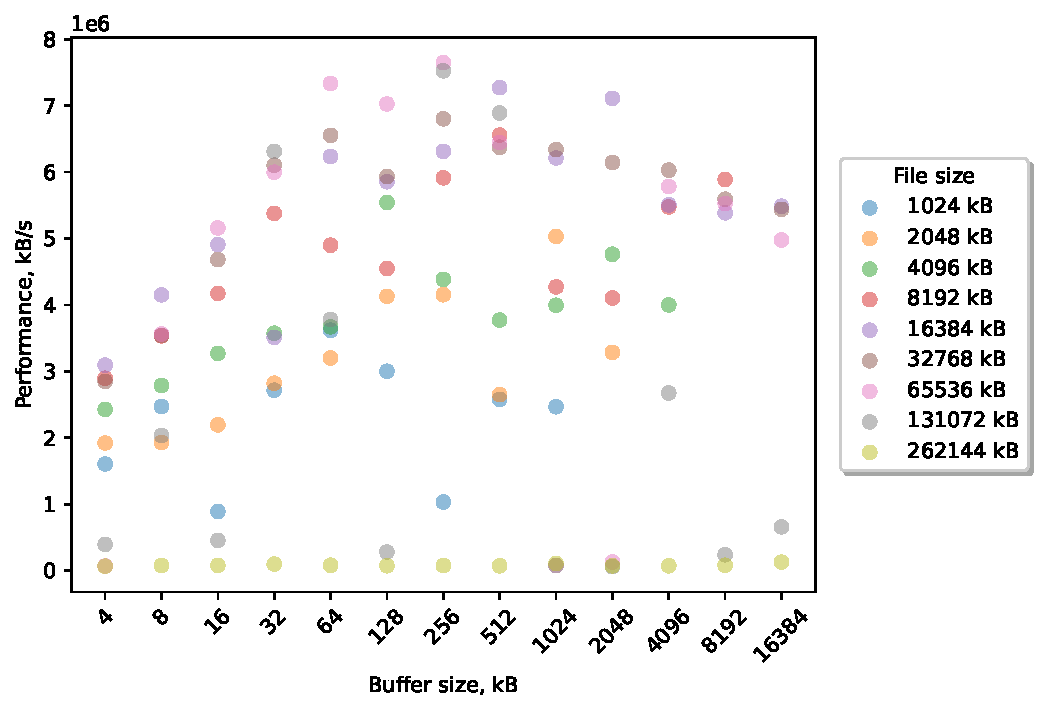
\includegraphics[width=1.0\textwidth]{figures.nosync/benchmarking/old/fejk-ffs/Read.pdf}
% 	\end{center}
% 	\caption{IOZone output for Fejk FFS Forward Read}
% \end{figure}

% \begin{figure}[!htb]
% 	\label{fig:app_benchf_ffs_write}
% 	\begin{center}
% 		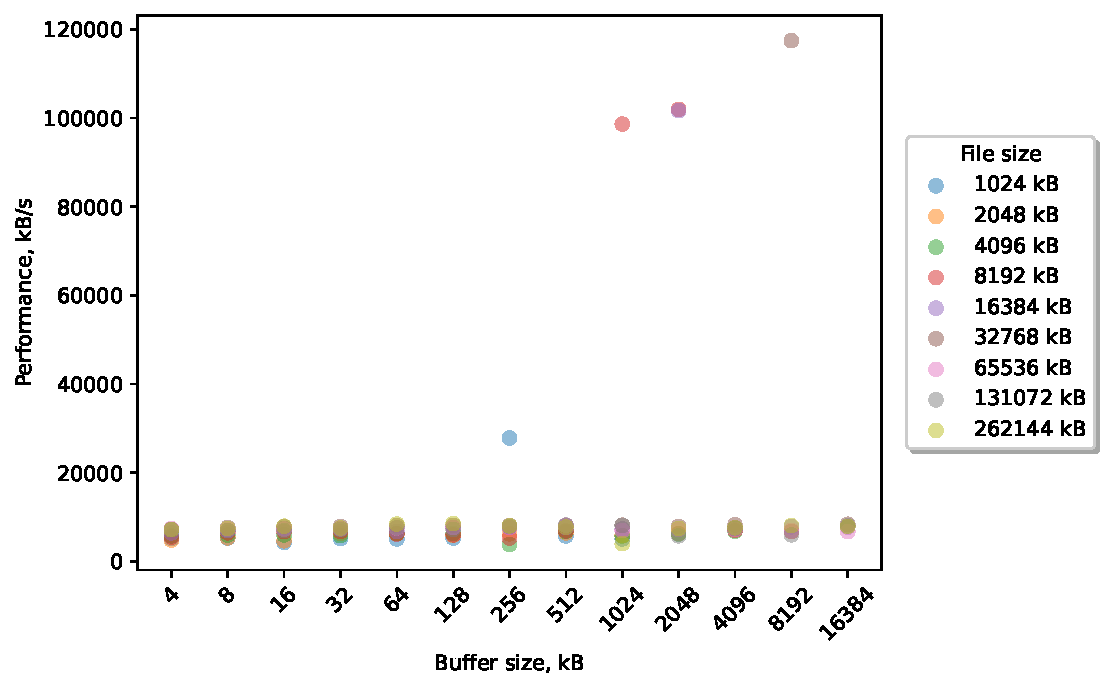
\includegraphics[width=1.0\textwidth]{figures.nosync/benchmarking/old/fejk-ffs/Write.pdf}
% 	\end{center}
% 	\caption{IOZone output for Fejk FFS Forward Write}
% \end{figure}

% \begin{figure}[!htb]
% 	\label{fig:app_bench_fffs_re_read}
% 	\begin{center}
% 		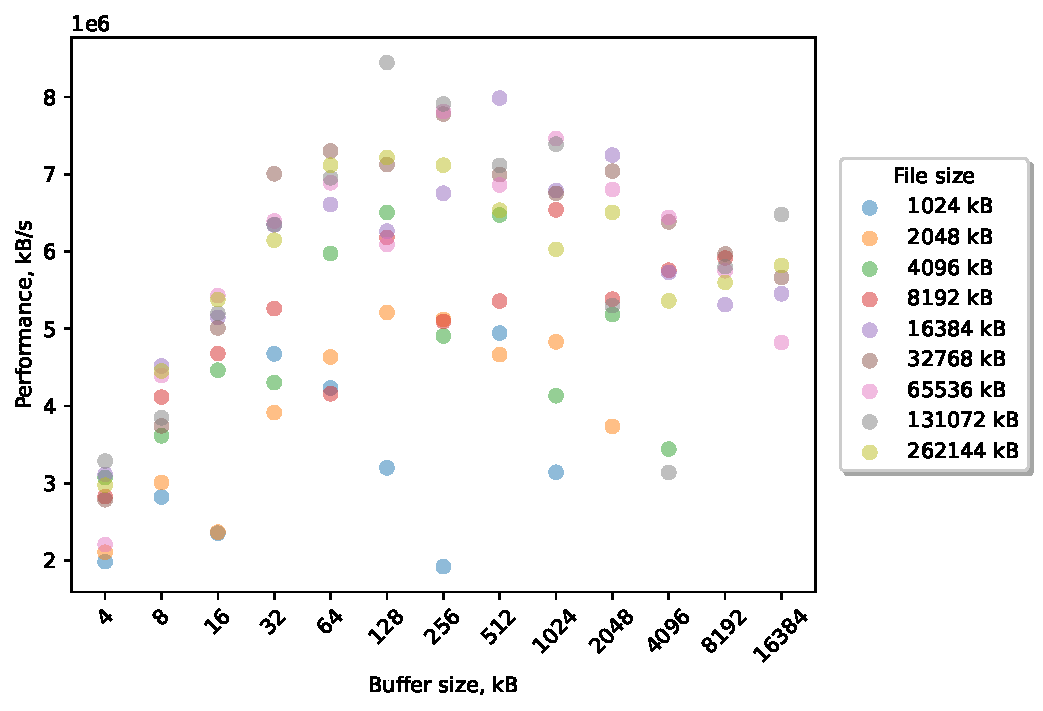
\includegraphics[width=1.0\textwidth]{figures.nosync/benchmarking/old/fejk-ffs/Re-Read.pdf}
% 	\end{center}
% 	\caption{IOZone output for Fejk FFS \mbox{Re-Read}}
% \end{figure}

% \begin{figure}[!htb]
% 	\label{fig:app_bench_fffs_re_write}
% 	\begin{center}
% 		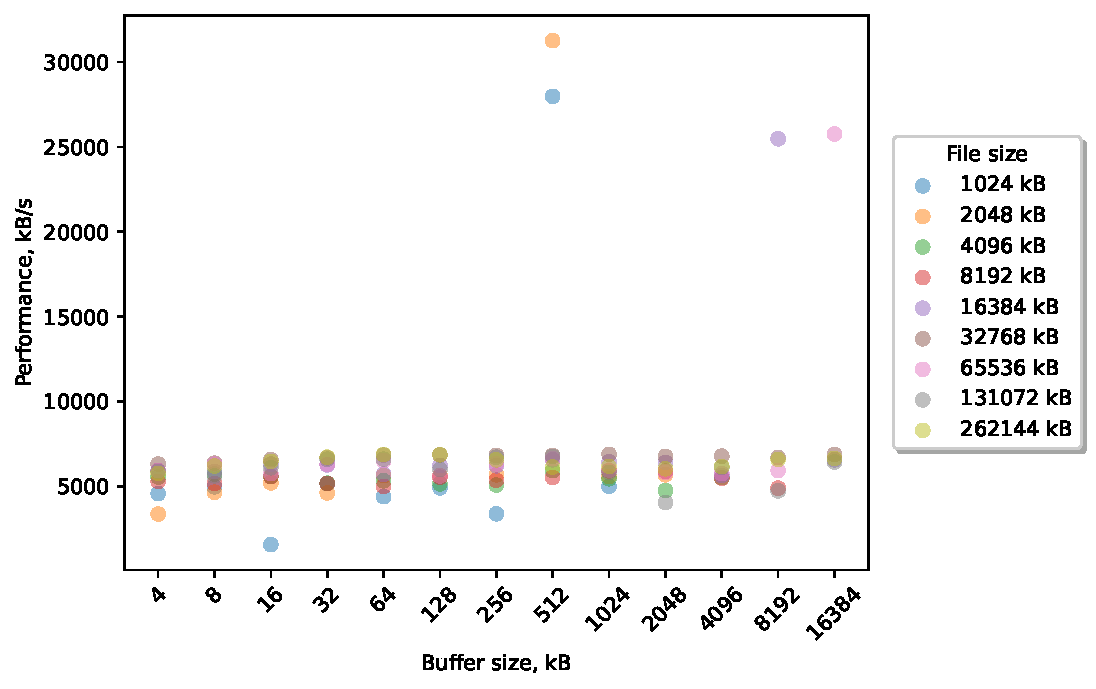
\includegraphics[width=1.0\textwidth]{figures.nosync/benchmarking/old/fejk-ffs/Re-Write.pdf}
% 	\end{center}
% 	\caption{IOZone output for Fejk FFS \mbox{Re-Write}}
% \end{figure}

% \begin{figure}[!htb]
% 	\label{fig:app_bench_fffs_rnd_read}
% 	\begin{center}
% 		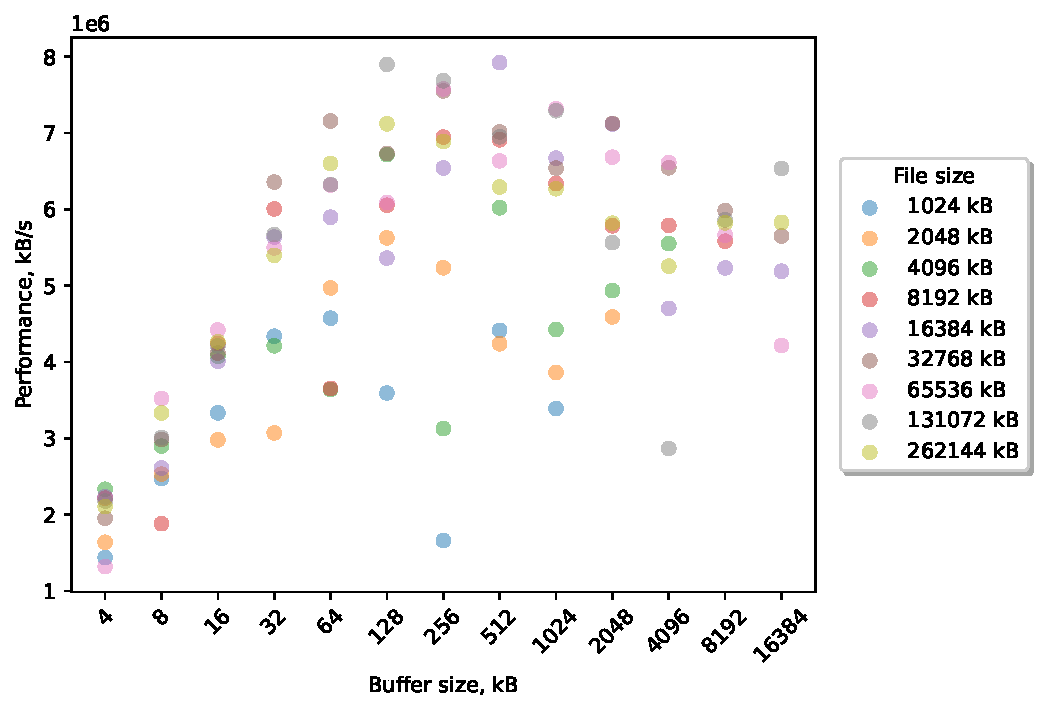
\includegraphics[width=1.0\textwidth]{figures.nosync/benchmarking/old/fejk-ffs/Random read.pdf}
% 	\end{center}
% 	\caption{IOZone output for Fejk FFS Random read}
% \end{figure}

% \begin{figure}[!htb]
% 	\label{fig:app_bench_ffsf_rnd_write}
% 	\begin{center}
% 		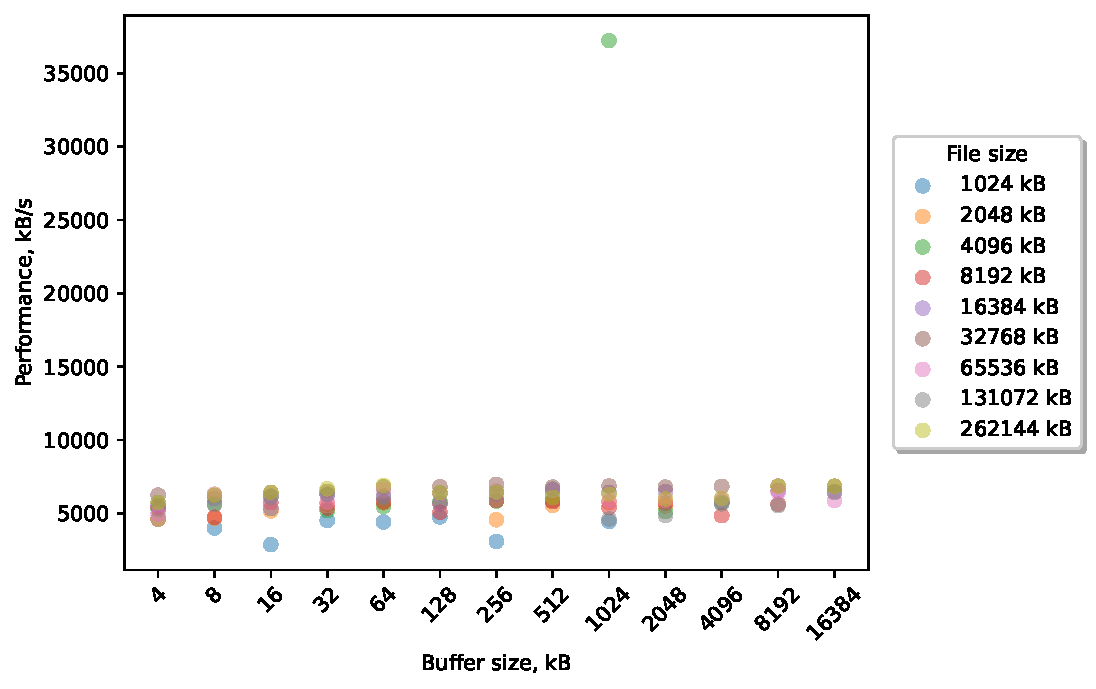
\includegraphics[width=1.0\textwidth]{figures.nosync/benchmarking/old/fejk-ffs/Random write.pdf}
% 	\end{center}
% 	\caption{IOZone output for Fejk FFS Random write}
% \end{figure}
\newpage

\section{APFS}

\begin{table}[!ht]
	\begin{center}
		\caption{IOZone result for the Read test on APFS in kilobytes per second}
		\resizebox{\textwidth}{!}{\begin{tabular}{| r | r | r | r | r | r | r | r | r | r | r | r | r | r | }
			
			\hline
			{} & \multicolumn{13}{c |}{Buffer size (kB)} \\
			\textbf{File size (kB)}   & \multicolumn{1}{c |}{4} & \multicolumn{1}{c |}{8} & \multicolumn{1}{c |}{16} & \multicolumn{1}{c |}{32} & \multicolumn{1}{c |}{64} & \multicolumn{1}{c |}{128} & \multicolumn{1}{c |}{256} & \multicolumn{1}{c |}{512} & \multicolumn{1}{c |}{1024} & \multicolumn{1}{c |}{2048} & \multicolumn{1}{c |}{4096} & \multicolumn{1}{c |}{8192} & \multicolumn{1}{c |}{16384}\\
			\hline
			\hline
			\textbf{1024}  & 538364 & 3908759 & 4488860 & 6128613 & 5251818 & 5660167 & 6402699 & 7420395 & 8474583 & {} & {} & {} & {}\\
			\textbf{2048}  & 2582813 & 3379461 & 4172290 & 5644567 & 5184636 & 6583305 & 5280246 & 6603549 & 8159088 & 7393606 & {} & {} & {}\\
			\textbf{4096}  & 2523925 & 3846119 & 4591331 & 5918366 & 6459069 & 6225028 & 6471234 & 5728903 & 7085049 & 6198078 & 5558378 & {} & {}\\
			\textbf{8192}  & 2689438 & 3653812 & 4902367 & 5603526 & 6081578 & 6310553 & 6720329 & 6809564 & 7067279 & 7154097 & 5422249 & 5776876 & {}\\
			\textbf{16384}  & 2675387 & 3779365 & 5457909 & 6347747 & 7440550 & 6818216 & 7702417 & 3990259 & 6054683 & 6367155 & 6698584 & 5477922 & 5027467\\
			\textbf{32768}  & 2654604 & 4438267 & 5507073 & 6566975 & 4920870 & 6247564 & 6546954 & 6621073 & 5274791 & 7583338 & 2896268 & 5498920 & 5641806\\
			\textbf{65536}  & 2574587 & 4011012 & 4825568 & 5732617 & 6554261 & 6607037 & 6608467 & 6864601 & 6640556 & 6608467 & 4768972 & 5492416 & 5470445\\
			\textbf{131072}  & 2665860 & 3968043 & 5421344 & 5545873 & 5938696 & 6221082 & 6147894 & 6289118 & 6388735 & 2839445 & 3350171 & 5215562 & 4865147\\
			\textbf{262144}  & 2385943 & 2904121 & 4293712 & 5289093 & 4596201 & 6348519 & 6435168 & 7442619 & 7397503 & 7744086 & 6419575 & 5641535 & 3369068\\


			\hline

		\end{tabular}}
		\label{tbl:data_local_read}
	\end{center}
\end{table}
	
\begin{table}[!ht]
	\begin{center}
		\caption{IOZone result for the Write test on APFS in kilobytes per second}
		\resizebox{\textwidth}{!}{\begin{tabular}{| r | r | r | r | r | r | r | r | r | r | r | r | r | r | }
			
			\hline
			{} & \multicolumn{13}{c |}{Buffer size (kB)} \\
			\textbf{File size (kB)}   & \multicolumn{1}{c |}{4} & \multicolumn{1}{c |}{8} & \multicolumn{1}{c |}{16} & \multicolumn{1}{c |}{32} & \multicolumn{1}{c |}{64} & \multicolumn{1}{c |}{128} & \multicolumn{1}{c |}{256} & \multicolumn{1}{c |}{512} & \multicolumn{1}{c |}{1024} & \multicolumn{1}{c |}{2048} & \multicolumn{1}{c |}{4096} & \multicolumn{1}{c |}{8192} & \multicolumn{1}{c |}{16384}\\
			\hline
			\hline
			\textbf{1024}  & 186358 & 335392 & 512232 & 827258 & 699870 & 1032244 & 1273788 & 1477555 & 873705 & {} & {} & {} & {}\\
			\textbf{2048}  & 229598 & 236085 & 291779 & 397593 & 892849 & 514465 & 513420 & 574009 & 1394966 & 1341170 & {} & {} & {}\\
			\textbf{4096}  & 190955 & 306150 & 512697 & 562558 & 593887 & 959243 & 806157 & 867415 & 754866 & 642314 & 1117622 & {} & {}\\
			\textbf{8192}  & 169441 & 255864 & 357293 & 401784 & 651754 & 675577 & 650779 & 675976 & 564729 & 633023 & 708889 & 752384 & {}\\
			\textbf{16384}  & 229954 & 310425 & 353652 & 491394 & 722178 & 716747 & 601890 & 639573 & 775984 & 708683 & 579081 & 698945 & 784336\\
			\textbf{32768}  & 201952 & 299576 & 431731 & 562454 & 584277 & 593696 & 609775 & 421778 & 769363 & 662034 & 427841 & 483047 & 741123\\
			\textbf{65536}  & 205960 & 323049 & 351173 & 451792 & 416014 & 504320 & 495422 & 632520 & 336679 & 473751 & 501468 & 662240 & 523098\\
			\textbf{131072}  & 210777 & 300665 & 358868 & 352807 & 399321 & 527975 & 431966 & 419926 & 413309 & 349982 & 282681 & 307020 & 224134\\
			\textbf{262144}  & 213134 & 286667 & 418873 & 410737 & 231669 & 474854 & 322547 & 305477 & 446954 & 702936 & 283134 & 563923 & 396791\\


			\hline

		\end{tabular}}
		\label{tbl:data_local_write}
	\end{center}
\end{table}
	
\begin{table}[!ht]
	\begin{center}
		\caption{IOZone result for the Re-Read test on APFS in kilobytes per second}
		\resizebox{\textwidth}{!}{\begin{tabular}{| r | r | r | r | r | r | r | r | r | r | r | r | r | r | }
			
			\hline
			{} & \multicolumn{13}{c |}{Buffer size (kB)} \\
			\textbf{File size (kB)}   & \multicolumn{1}{c |}{4} & \multicolumn{1}{c |}{8} & \multicolumn{1}{c |}{16} & \multicolumn{1}{c |}{32} & \multicolumn{1}{c |}{64} & \multicolumn{1}{c |}{128} & \multicolumn{1}{c |}{256} & \multicolumn{1}{c |}{512} & \multicolumn{1}{c |}{1024} & \multicolumn{1}{c |}{2048} & \multicolumn{1}{c |}{4096} & \multicolumn{1}{c |}{8192} & \multicolumn{1}{c |}{16384}\\
			\hline
			\hline
			\textbf{1024}  & 2942149 & 4300102 & 4898425 & 7420395 & 8000971 & 6918376 & 8970167 & 8199542 & 10662628 & {} & {} & {} & {}\\
			\textbf{2048}  & 2892423 & 4038890 & 4911886 & 9101380 & 6967792 & 8059569 & 4284671 & 8464610 & 9898453 & 10660056 & {} & {} & {}\\
			\textbf{4096}  & 2603876 & 3991785 & 4853336 & 6330545 & 7380284 & 6669706 & 7355007 & 7135072 & 7515892 & 6625976 & 5744227 & {} & {}\\
			\textbf{8192}  & 2578436 & 3948121 & 5047109 & 6118398 & 6627005 & 6855760 & 7205103 & 7386322 & 7474698 & 8152152 & 4955393 & 5013234 & {}\\
			\textbf{16384}  & 2666252 & 3689278 & 5628220 & 6660280 & 7736235 & 7050461 & 8087683 & 3954666 & 5923170 & 6405137 & 5624535 & 5472251 & 4733787\\
			\textbf{32768}  & 2459325 & 4444294 & 5092820 & 6114429 & 5524116 & 6207215 & 6885441 & 6739910 & 5866989 & 6999048 & 2186853 & 5164391 & 5674182\\
			\textbf{65536}  & 2609539 & 3811988 & 4921646 & 5591403 & 6577945 & 6843750 & 6577315 & 7125655 & 7737415 & 6903565 & 4937914 & 5074468 & 5140421\\
			\textbf{131072}  & 2795139 & 3709708 & 5510463 & 5775607 & 6114321 & 6257620 & 5947047 & 6486732 & 5777367 & 2253302 & 2813722 & 4947994 & 4669283\\
			\textbf{262144}  & 2259139 & 3316468 & 3623921 & 4864863 & 5380721 & 6522434 & 7086865 & 7440101 & 6565902 & 6814965 & 6387391 & 5202306 & 4402011\\


			\hline

		\end{tabular}}
		\label{tbl:data_local_re-read}
	\end{center}
\end{table}
	
\begin{table}[!ht]
	\begin{center}
		\caption{IOZone result for the Re-Write test on APFS in kilobytes per second}
		\resizebox{\textwidth}{!}{\begin{tabular}{| r | r | r | r | r | r | r | r | r | r | r | r | r | r | }
			
			\hline
			{} & \multicolumn{13}{c |}{Buffer size (kB)} \\
			\textbf{File size (kB)}   & \multicolumn{1}{c |}{4} & \multicolumn{1}{c |}{8} & \multicolumn{1}{c |}{16} & \multicolumn{1}{c |}{32} & \multicolumn{1}{c |}{64} & \multicolumn{1}{c |}{128} & \multicolumn{1}{c |}{256} & \multicolumn{1}{c |}{512} & \multicolumn{1}{c |}{1024} & \multicolumn{1}{c |}{2048} & \multicolumn{1}{c |}{4096} & \multicolumn{1}{c |}{8192} & \multicolumn{1}{c |}{16384}\\
			\hline
			\hline
			\textbf{1024}  & 718605 & 1095150 & 1207534 & 2174880 & 2011877 & 2391665 & 2681328 & 2877110 & 2516377 & {} & {} & {} & {}\\
			\textbf{2048}  & 659151 & 717873 & 1276781 & 1728076 & 1642495 & 2228370 & 2324867 & 2144371 & 2479196 & 2164908 & {} & {} & {}\\
			\textbf{4096}  & 575755 & 815146 & 1035380 & 1213970 & 1113926 & 1490556 & 1442740 & 1410868 & 1140927 & 1656880 & 1293391 & {} & {}\\
			\textbf{8192}  & 465744 & 595615 & 743978 & 799606 & 902996 & 928069 & 952326 & 957100 & 929425 & 967176 & 944862 & 862231 & {}\\
			\textbf{16384}  & 477530 & 623578 & 762230 & 829106 & 809485 & 828646 & 866283 & 863811 & 854137 & 861904 & 818997 & 844138 & 791153\\
			\textbf{32768}  & 462407 & 643152 & 739050 & 789018 & 812878 & 810386 & 816665 & 794817 & 803352 & 805249 & 454334 & 770251 & 640425\\
			\textbf{65536}  & 471824 & 503414 & 594355 & 430945 & 498426 & 542350 & 460111 & 450153 & 507700 & 458117 & 460379 & 537131 & 437673\\
			\textbf{131072}  & 444825 & 469368 & 259988 & 389394 & 424943 & 387612 & 395487 & 399679 & 394444 & 429177 & 350255 & 351668 & 373706\\
			\textbf{262144}  & 353860 & 289345 & 314443 & 372257 & 260874 & 429759 & 331707 & 450561 & 473636 & 535371 & 457672 & 544259 & 480567\\


			\hline

		\end{tabular}}
		\label{tbl:data_local_re-write}
	\end{center}
\end{table}
	
\begin{table}[!ht]
	\begin{center}
		\caption{IOZone result for the Random read test on APFS in kilobytes per second}
		\resizebox{\textwidth}{!}{\begin{tabular}{| r | r | r | r | r | r | r | r | r | r | r | r | r | r | }
			
			\hline
			{} & \multicolumn{13}{c |}{Buffer size (kB)} \\
			\textbf{File size (kB)}   & \multicolumn{1}{c |}{4} & \multicolumn{1}{c |}{8} & \multicolumn{1}{c |}{16} & \multicolumn{1}{c |}{32} & \multicolumn{1}{c |}{64} & \multicolumn{1}{c |}{128} & \multicolumn{1}{c |}{256} & \multicolumn{1}{c |}{512} & \multicolumn{1}{c |}{1024} & \multicolumn{1}{c |}{2048} & \multicolumn{1}{c |}{4096} & \multicolumn{1}{c |}{8192} & \multicolumn{1}{c |}{16384}\\
			\hline
			\hline
			\textbf{1024}  & 2159571 & 3229770 & 5593820 & 6744549 & 6519323 & 7485055 & 8076196 & 6393168 & 7257394 & {} & {} & {} & {}\\
			\textbf{2048}  & 2209455 & 3418463 & 4170264 & 7789164 & 6967792 & 9140117 & 4531020 & 8325147 & 9189005 & 7582884 & {} & {} & {}\\
			\textbf{4096}  & 2004931 & 3407483 & 4262142 & 6512939 & 7355007 & 6953144 & 7892238 & 7756829 & 7863339 & 6300364 & 5679660 & {} & {}\\
			\textbf{8192}  & 1944875 & 2874376 & 4248864 & 5565406 & 6434642 & 6736139 & 6481984 & 6470997 & 7772279 & 7786370 & 5287898 & 6006101 & {}\\
			\textbf{16384}  & 1991764 & 2995773 & 4687931 & 5736755 & 6622411 & 6764523 & 7918992 & 4595758 & 5809993 & 6609036 & 6924710 & 5659275 & 4982992\\
			\textbf{32768}  & 1767526 & 3215713 & 4479493 & 5964247 & 5520123 & 4968725 & 6777467 & 6518388 & 6288441 & 7759298 & 928793 & 4964956 & 5361210\\
			\textbf{65536}  & 1900469 & 2952349 & 4178758 & 5048558 & 5798157 & 6123665 & 6282233 & 7567639 & 7736326 & 6572597 & 4738064 & 5052920 & 4938268\\
			\textbf{131072}  & 1973295 & 2972025 & 4590640 & 5011365 & 5677078 & 5602332 & 5535598 & 6621505 & 4934581 & 2565107 & 2293317 & 4654537 & 4205861\\
			\textbf{262144}  & 1645466 & 2529888 & 3703645 & 4595951 & 5555647 & 5328877 & 6941457 & 5965271 & 6178287 & 5808891 & 6445013 & 5152113 & 3875397\\


			\hline

		\end{tabular}}
		\label{tbl:data_local_random_read}
	\end{center}
\end{table}
	
\begin{table}[!ht]
	\begin{center}
		\caption{IOZone result for the Random write test on APFS in kilobytes per second}
		\resizebox{\textwidth}{!}{\begin{tabular}{| r | r | r | r | r | r | r | r | r | r | r | r | r | r | }
			
			\hline
			{} & \multicolumn{13}{c |}{Buffer size (kB)} \\
			\textbf{File size (kB)}   & \multicolumn{1}{c |}{4} & \multicolumn{1}{c |}{8} & \multicolumn{1}{c |}{16} & \multicolumn{1}{c |}{32} & \multicolumn{1}{c |}{64} & \multicolumn{1}{c |}{128} & \multicolumn{1}{c |}{256} & \multicolumn{1}{c |}{512} & \multicolumn{1}{c |}{1024} & \multicolumn{1}{c |}{2048} & \multicolumn{1}{c |}{4096} & \multicolumn{1}{c |}{8192} & \multicolumn{1}{c |}{16384}\\
			\hline
			\hline
			\textbf{1024}  & 653942 & 1121751 & 1758930 & 2295784 & 2461573 & 2086145 & 3259181 & 3301774 & 3229770 & {} & {} & {} & {}\\
			\textbf{2048}  & 651403 & 941176 & 1615011 & 2235328 & 2622235 & 2972495 & 1903457 & 2694623 & 2756005 & 3256469 & {} & {} & {}\\
			\textbf{4096}  & 530639 & 717717 & 914318 & 1314470 & 1365344 & 1659601 & 1665715 & 1479262 & 1127080 & 1445410 & 1332929 & {} & {}\\
			\textbf{8192}  & 519368 & 735363 & 998544 & 1222122 & 1447895 & 1400334 & 1472909 & 1523253 & 985796 & 968649 & 934531 & 808924 & {}\\
			\textbf{16384}  & 421455 & 596907 & 756066 & 866599 & 873862 & 962622 & 989541 & 903290 & 964053 & 959142 & 1011178 & 829827 & 830368\\
			\textbf{32768}  & 385047 & 544336 & 662903 & 742733 & 766501 & 778374 & 810807 & 804240 & 798655 & 807050 & 695475 & 795015 & 794009\\
			\textbf{65536}  & 325765 & 398351 & 434435 & 461241 & 520668 & 518300 & 488421 & 525891 & 542606 & 525094 & 562661 & 623386 & 461969\\
			\textbf{131072}  & 271885 & 299055 & 309948 & 369675 & 422510 & 435145 & 406463 & 422968 & 442190 & 330912 & 366528 & 363675 & 471680\\
			\textbf{262144}  & 247316 & 294339 & 301800 & 336086 & 262214 & 410092 & 337473 & 365472 & 497358 & 449168 & 418914 & 544169 & 657338\\


			\hline

		\end{tabular}}
		\label{tbl:data_local_random_write}
	\end{center}
\end{table}
	

\FloatBarrier
% \begin{figure}[!htb]
% 	\label{fig:app_beapfs_ffs_read}
% 	\begin{center}
% 		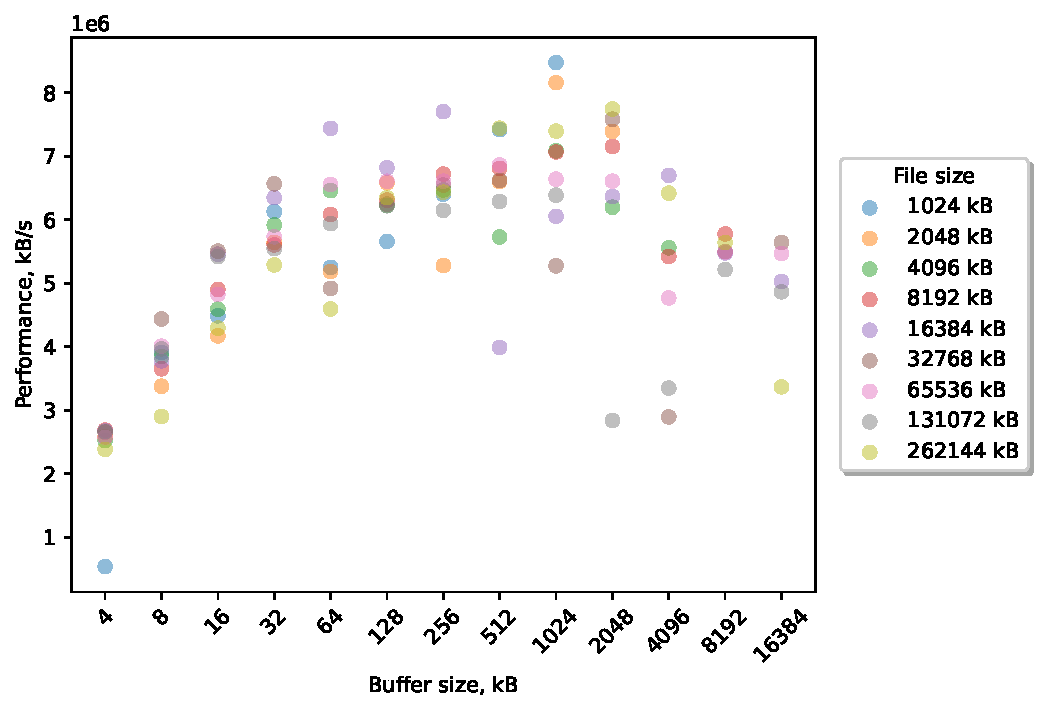
\includegraphics[width=1.0\textwidth]{figures.nosync/benchmarking/old/local/Read.pdf}
% 	\end{center}
% 	\caption{IOZone output for \gls{APFS} Forward Read}
% \end{figure}

% \begin{figure}[!htb]
% 	\label{fig:app_benapfsffs_write}
% 	\begin{center}
% 		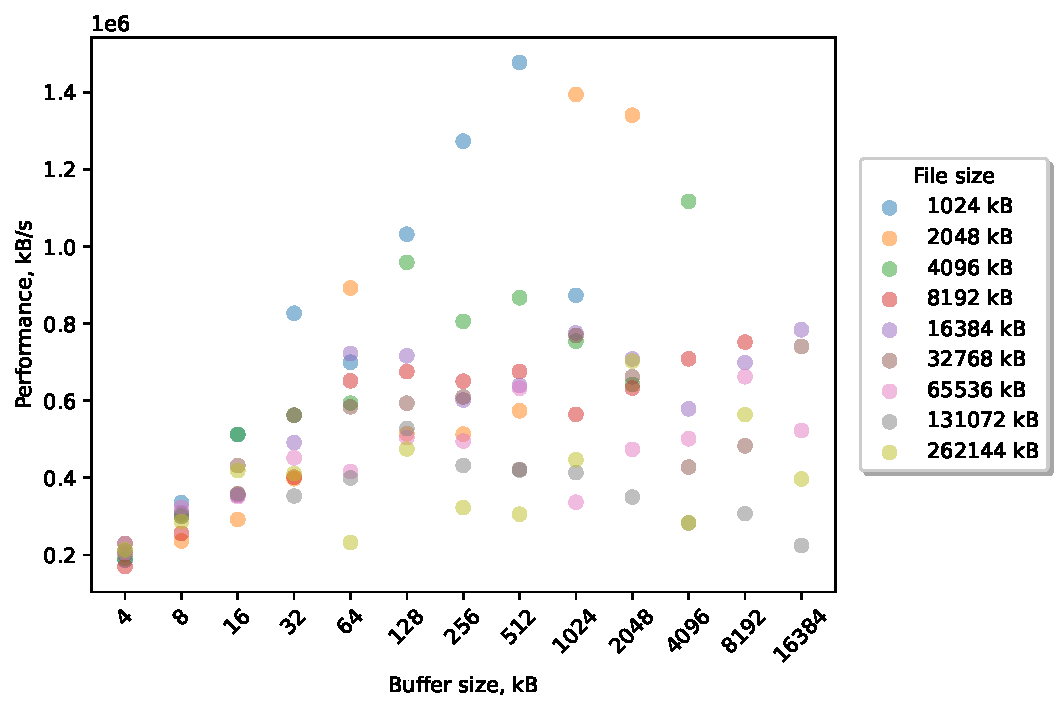
\includegraphics[width=1.0\textwidth]{figures.nosync/benchmarking/old/local/Write.pdf}
% 	\end{center}
% 	\caption{IOZone output for \gls{APFS} Forward Write}
% \end{figure}

% \begin{figure}[!htb]
% 	\label{fig:app_benchapfss_re_read}
% 	\begin{center}
% 		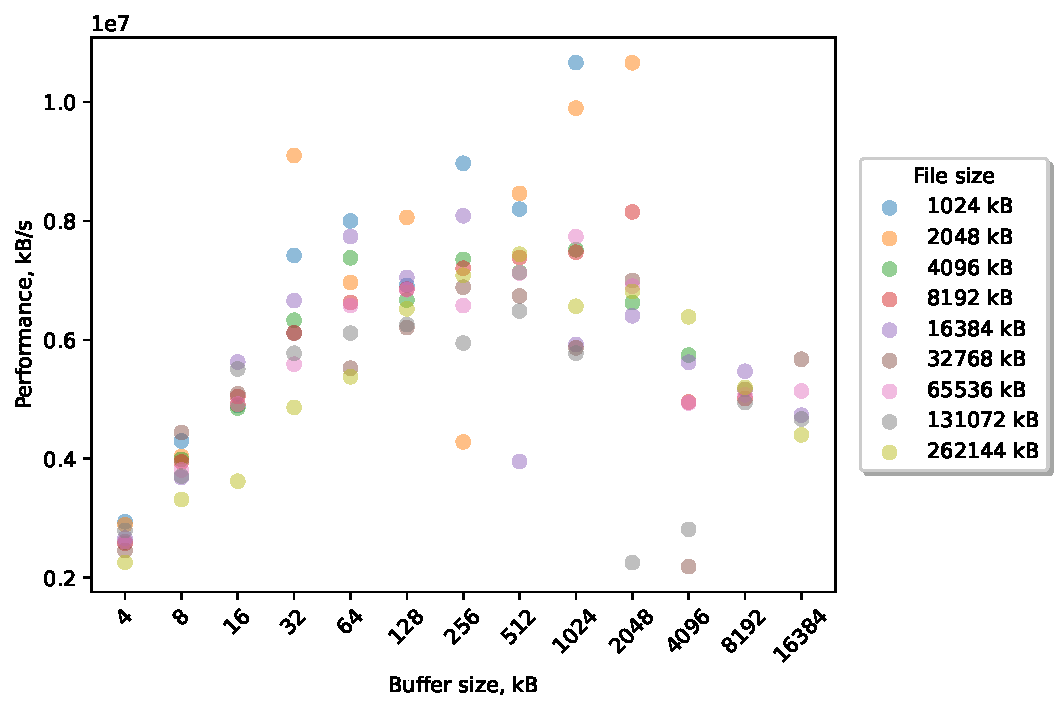
\includegraphics[width=1.0\textwidth]{figures.nosync/benchmarking/old/local/Re-Read.pdf}
% 	\end{center}
% 	\caption{IOZone output for \gls{APFS} \mbox{Re-Read}}
% \end{figure}

% \begin{figure}[!htb]
% 	\label{fig:app_bench_apfs_re_write}
% 	\begin{center}
% 		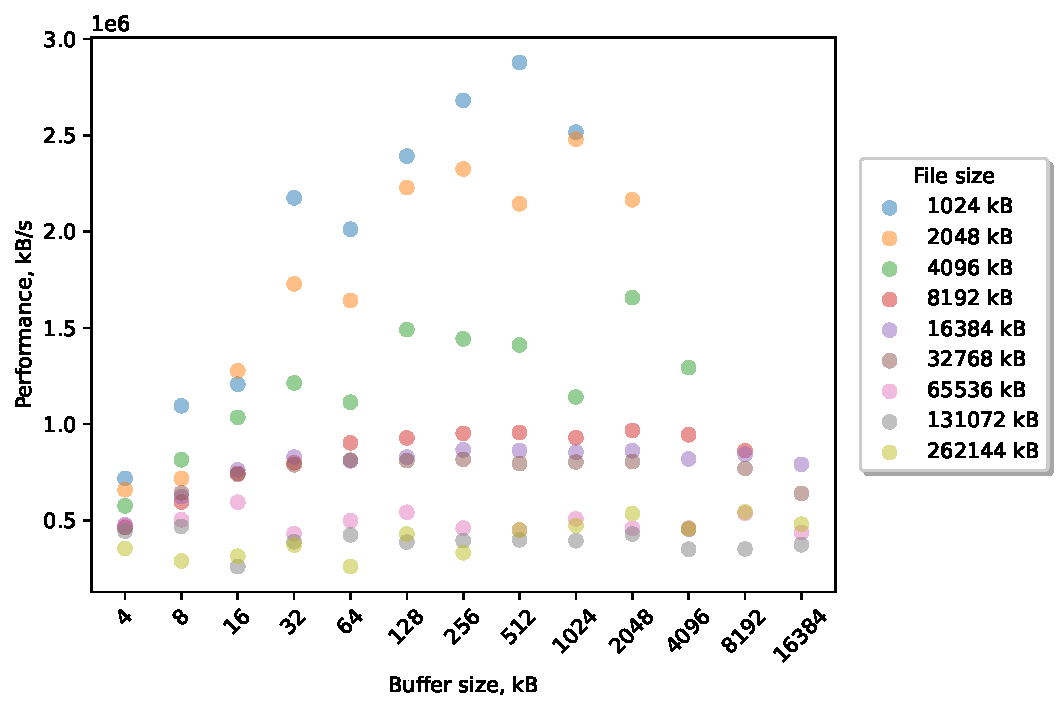
\includegraphics[width=1.0\textwidth]{figures.nosync/benchmarking/old/local/Re-Write.pdf}
% 	\end{center}
% 	\caption{IOZone output for \gls{APFS} \mbox{Re-Write}}
% \end{figure}

% \begin{figure}[!htb]
% 	\label{fig:app_bench_apfs_rnd_read}
% 	\begin{center}
% 		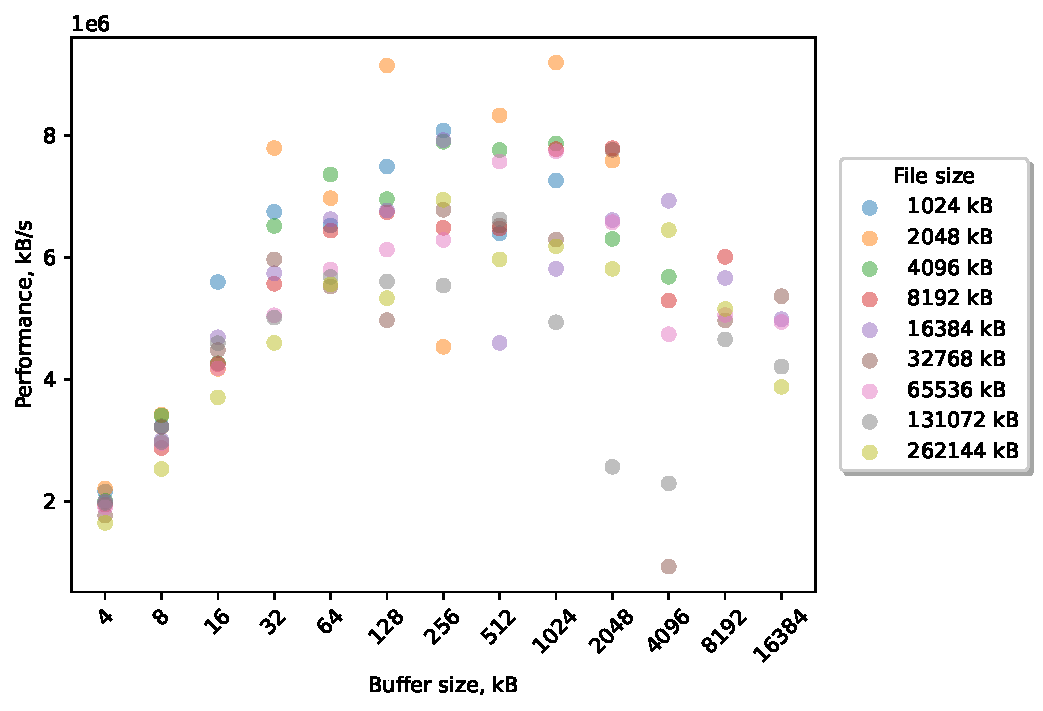
\includegraphics[width=1.0\textwidth]{figures.nosync/benchmarking/old/local/Random read.pdf}
% 	\end{center}
% 	\caption{IOZone output for \gls{APFS} Random read}
% \end{figure}

% \begin{figure}[!htb]
% 	\label{fig:app_bench_fapfsrnd_write}
% 	\begin{center}
% 		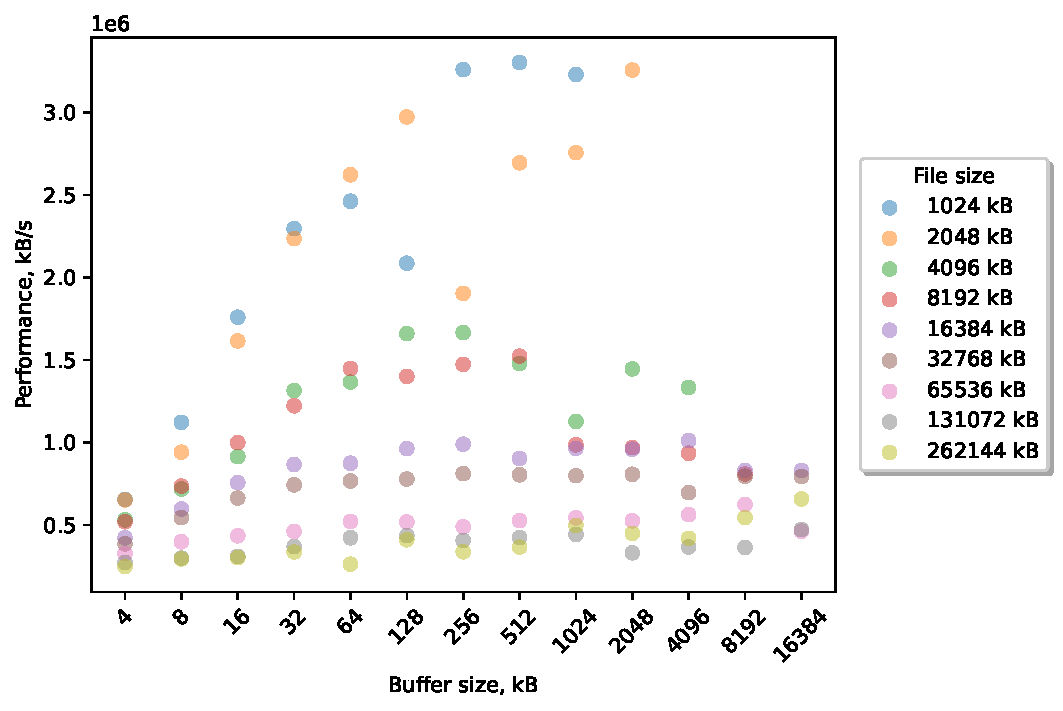
\includegraphics[width=1.0\textwidth]{figures.nosync/benchmarking/old/local/Random write.pdf}
% 	\end{center}
% 	\caption{IOZone output for \gls{APFS} Random write}
% \end{figure}